%%%%%%%%%%%%%%%%%%%%%%%%%%%%%%%%%%%%%%%%%%
% Engineering problems / LaTeX Template
%		Semester 5
%		Institut d'Optique Graduate School
%%%%%%%%%%%%%%%%%%%%%%%%%%%%%%%%%%%%%%%%%%
%	5N-OptoElec-Bloc1	/ caractérisation statique
%%%%%%%%%%%%%%%%%%%%%%%%%%%%%%%%%%%%%%%%%%
%
% Created by:
%	Julien VILLEMEJANE - 16/jul/2024
% Modified by: 06/09/24 
%	
%
%%%%%%%%%%%%%%%%%%%%%%%%%%%%%%%%%%%%%%%%%%
% Professional Newsletter Template
% LaTeX Template
% Version 1.0 (09/03/14)
%
% Created by:
% Bob Kerstetter (https://www.tug.org/texshowcase/) and extensively modified by:
% Vel (vel@latextemplates.com)
% 
% This template has been downloaded from:
% http://www.LaTeXTemplates.com
%
% License:
% CC BY-NC-SA 3.0 (http://creativecommons.org/licenses/by-nc-sa/3.0/)
%
%%%%%%%%%%%%%%%%%%%%%%%%%%%%%%%%%%%%%%%%%

\documentclass[a4paper,11pt,twoside]{book} % The default font size is 10pt; 11pt and 12pt are alternatives

\usepackage{opto_elec_villemejane}


%%%%%%%%%%%%%%%%%%%%%%%%%%%%%%%%%%%%%%%%%%%%%%%%
%%%%%%%%%%%%%%%%%%%%%%%%%%%%%%%%%%%%%%%%%%%%%%%%
%%%%%%%%%%%%%%%%%%%%%%%%%%%%%%%%%%%%%%%%%%%%%%%%
%%%%%%%%%%%%%%%%%%%%%%%%%%%%%%%%%%%%%%%%%%%%%%%%
\begin{document}


% Page de garde
\begin{titlepage}

\begin{center}
	\begin{minipage}{2.5cm}
	\begin{center}
		
\includegraphics[width=8cm]{images/Logo-LEnsE.png}
	\end{center}
\end{minipage}\hfill
\begin{minipage}{10cm}
	\begin{center}
	\textbf{Institut d'Optique Graduate School }\\[0.1cm]
    \textbf{TP d'Opto-Électronique}


	\end{center}
\end{minipage}\hfill


\vspace{1.0cm}


{\huge \bfseries \textsc{Opto-Électronique}} \\[0.5cm]
{\large \bfseries Travaux Pratiques} \\[0.2cm]
Semestre 5

\vspace{0.5cm}
% Title
\rule{\linewidth}{0.3mm} \\[0.4cm]
{ \huge \bfseries\color{violet_iogs} Notions et Protocoles \\[0.4cm] }
\rule{\linewidth}{0.3mm} \\[1cm]


{\large \textbf{Protocoles}}

\begin{itemize}[label=$\blacktriangleright$]
	\item \hyperref[ressource:CaracStat]{Tracer la \textbf{caractéristique statique} d'un dipôle}
	\item \hyperref[ressource:RepIndic]{Tracer la \textbf{réponse indicielle} d'un système linéaire}
	\item \hyperref[ressource:RepFreq]{Tracer la \textbf{réponse en fréquence} d'un système linéaire (\textbf{gain} et \textbf{phase})}
	\item \hyperref[ressource:BandePassante]{Mesurer la \textbf{bande passante} d'un système linéaire}
\end{itemize}

\medskip


{\large \textbf{Notions}}

\begin{itemize}[label=$\blacktriangleright$]
	\item \hyperref[fiche:Bases1]{Réseaux et Dipôles}
	\item \hyperref[fiche:Bases2]{Systèmes linéaires et Superposition}
	\item \hyperref[fiche:Capteurs]{Capteurs}
	\item \hyperref[fiche:LED]{Diode, LED et photodiode}
	\item \hyperref[fiche:Photodetection]{Photodétection}
	\item \hyperref[fiche:ALI]{Amplificateur Linéaire Intégré / Principe et montages de base}
	\item \hyperref[fiche:ALIModele]{Amplificateur Linéaire Intégré / Modélisation et rebouclage}
	\item \hyperref[fiche:RegimeHarmonique]{Régime Harmonique}
	\item \hyperref[fiche:AnHaOrdre1]{Filtrage / Analyse harmonique / Ordre 1}
	\item \hyperref[fiche:AnHaOrdre2]{Filtrage / Analyse harmonique / Ordre 2}	
	\item \hyperref[fiche:ModeleTransimpedance]{Systèmes bouclés simples / Exemple du transimpédance}
	
\end{itemize}


\bigskip

\textit{Ce document est disponible au format électronique sur le site du LEnsE - https://lense.institutoptique.fr/ dans la rubrique Année / Première Année / Opto-Electronique S5 / TP / Notions et Protocoles.}

\medskip

\begin{minipage}{5cm}
\begin{center}

\includegraphics[width=3cm]{./images/logocc}\\
\small
  © 2025 by LEnsE-IOGS 
\end{center}
\end{minipage}


\end{center}
\end{titlepage}



% ----- DEUXIÈME PAGE (sans numérotation) -----
\clearpage
\thispagestyle{empty}
\mbox{} % page vide ou mettre du texte si souhaité

% ----- TROISIÈME PAGE (début de la numérotation à 1) -----
\clearpage
\setcounter{page}{1} % on commence la numérotation ici
\pagenumbering{arabic} % pour utiliser les chiffres arabes
\pagestyle{plain} % ou autre style si souhaité
  

% Protocoles
\newpage
\pagestyle{empty}

\begin{minipage}[c]{.25\linewidth}
	
\includegraphics[width=4cm]{images/Logo-LEnsE.png}
\end{minipage} \hfill
\begin{minipage}[c]{.4\linewidth}

\begin{center}
\vspace{0.3cm}
{\Large \textsc{Opto-Électronique}}

\medskip

\textbf{\Large Ressources}

\end{center}
\end{minipage}\hfill

\vspace{0.5cm}

\noindent \rule{\linewidth}{1pt}
\section{Caractéristique statique d'un dipôle}
\label{ressource:CaracStat}


%%%%%%%%%%%%%%%%%%%%%%%%%%%%%%%%%%%%%%%%%%%%%%%%%%%%%%%%%%%%%%%%%%%%%%%%%%%%%%%%
%%%%%

En électronique, la caractéristique statique d'un dipôle correspond à la relation mathématique $i=f(u)$ qu'il existe entre la différence de potentiel $u$ à ses bornes et le courant $i$ le traversant, dans des conditions statiques, c'est-à-dire lorsque ces deux grandeurs ne sont pas dépendantes du temps.

\medskip

Il existe deux méthodes principales pour caractériser statiquement un dipôle :

\begin{itemize}
	\item \textbf{une méthode manuelle}, qui permet de tracer point à point cette courbe, en faisant varier $u$ aux bornes du dipôle et en mesurant $u$ et $i$ pour un certain nombre de points,
	\item \textbf{une méthode automatique}, qui permet d'obtenir de manière plus rapide une allure de la caractéristique statique sur un oscilloscope.
\end{itemize}


\subsection*{Caractéristique Manuelle}

Une première méthode pour pouvoir \textbf{tracer la caractéristique statique} $i=f(u)$ d'un dipôle est de faire varier la différence de potentiel à ses bornes de manière statique (i.e. très lente) et de mesurer la différence de potentiel $u$ aux bornes du dipôle, à l'aide d'un voltmètre, et le courant $i$ le traversant, à l'aide d'un ampèremètre, point par point.

\medskip

Pour \textbf{faire varier la différence de potentiel} aux bornes du dipôle, on pourra prendre une \textbf{alimentation stabilisée réglable}.

Pour \textbf{mesurer la différence de potentiel} aux bornes du dipôle, on pourra utiliser un multimètre en mode \textbf{voltmètre} câblé en parallèle du dipôle.

Pour \textbf{mesurer le courant} traversant le dipôle, on pourra utiliser un multimètre en mode \textbf{ampèremètre} câblé en série avec le dipôle.

\subsubsection*{Circuit de mesure}

\begin{multicols}{2}

On donne le schéma suivant pour mesurer à la fois le courant et la différence de potentiel aux bornes d'un dipôle (ici une diode).


\subsubsection*{Méthode de mesure}

On mesure à la fois le courant, à l'aide de l'ampèremètre branché en série, et la différence de potentiel aux bornes de la LED, à l'aide d'un voltmètre branché en parallèle.

\columnbreak

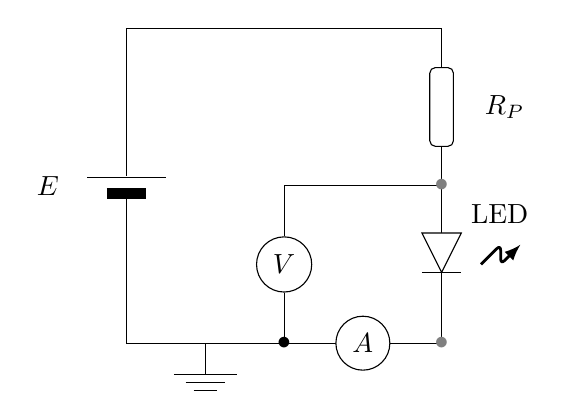
\begin{tikzpicture}
    \draw(0,-2)--(0,2)--(4,2)--(4,-2)--cycle;
    \node[fill=white, minimum height= 0.2cm] at (0,0) {}; 
    \draw(-0.5,0.1)--++(1,0);
    \draw[line width=4pt] (-0.25,-0.1)--++(0.5,0);
    
    
    %\draw[fill=white] (0,0) circle (0.5cm);
    %\draw [>=stealth, ->, very thick] (0,-0.25)--(0,0.25);
    \node at (-1,0) {$E$};
    \node[draw, fill=white, minimum width=0.3cm, minimum height=1cm, rounded corners =2pt] at (4,1) {};
    \node [xshift=0.8cm] at (4,1) {$R_{P}$};
    \draw(1,-2)--++(0,-0.4); \draw(0.6,-2.4)--++(0.8,0); \draw (0.75,-2.5)--++(0.5,0);\draw (0.85,-2.6)--++(0.3,0); 
    
    \node[circle,draw, fill =white](Voltmetre) at (2,-1) {$\operatorname{V}$};
    \draw (Voltmetre.north)|-(4,0) node[gray] {$\bullet$};
    \draw (Voltmetre.south)--(2,-2) node {$\bullet$};
    \node[circle,draw, fill =white](Ametre) at (3,-2) {$\operatorname{A}$};
    \node[gray] at (4,-2) {$\bullet$};

    %\draw (Ametre.east)--++(1,0) node (int) [midway]   {$\bullet$} --++(0,1) --++(0.4,0.8);
%\draw (0.5,2) -| (4.4,0.5);
%\draw (0.5,-1)  -|(Ametre.west);
%\draw (Voltmetre.north)--(2,2) node {$\bullet$};
%\draw (Voltmetre.south)--(2,-1) node {$\bullet$};

    
            \begin{scope}[xshift=3.75cm,yshift=-0.6cm]%LED
            \draw[fill=white] (0,0)--++(0.5,0)--++(-0.25,-0.5)--cycle;
            \draw (0,-0.5)--++(0.5,0) node[above right, yshift=0.5cm]{LED};
            \draw[->,>=latex,rounded corners=2pt, line width=1pt] (0.75,-0.4) --++ (0.25,0.25)--++(0,-0.25)--++(0.25,0.25);
            \node (A1) at (0.25,0) {};
            \node (K1) at (0.25,-0.5) {};
            \end{scope}        
\end{tikzpicture}

\end{multicols}


On fait alors varier le potentiel de la source de tension $E$, pour relever, pour plusieurs points, les valeurs du courant (A) et de la différence de potentiel (V).

La plupart des multimètres permettent d'afficher simultanément la tension et le courant continu.

Les points peuvent ensuite être enregistrés dans un fichier de tableur (type Excel ou Calc). Cet outil logiciel permettra par la suite de tracer la courbe $i=f(u)$.



\subsection*{Caractéristique Automatisée}

Une seconde méthode permettant d'\textbf{obtenir une allure de la caractéristique statique }$i=f(u)$ d'un dipôle est de faire varier la différence de potentiel à ses bornes en appliquant un signal dont l'amplitude varie lentement dans le temps. On peut alors mesurer la différence de potentiel $u$ aux bornes du dipôle et le courant $i$ le traversant à l'aide d'un oscilloscope en mode XY.

Cette méthode va nécessiter de \textbf{transformer le courant en différence de potentiel}, seule grandeur mesurable à l'aide d'un oscilloscope.

Pour faire \textbf{varier la différence de potentiel} aux bornes du dipôle, on utilisera une \textbf{générateur basse fréquence} (ou GBF).

Pour \textbf{mesurer la différence de potentiel} aux bornes du dipôle, on pourra utiliser une des voies de l'\textbf{oscilloscope} câblée en parallèle du dipôle.

Pour \textbf{mesurer le courant} traversant le dipôle, on insérera une \textbf{résistance de faible valeur} (afin de ne pas perturber le reste du montage par l'ajout d'un système de mesure) en série avec le dipôle que l'on cherche à caractériser. On pourra alors utiliser la seconde voie de l'\textbf{oscilloscope} pour mesurer la différence de potentiel aux bornes de cette résistance. Par la loi d'Ohms, on retrouvera alors la valeur du courant.

\subsubsection*{Circuit de mesure}

\begin{multicols}{2}

On donne le circuit suivant pour tracer de manière automatisée l'allure de la caractéristique statique.

\medskip


La résistance $R_P$ est une résistance de protection du dipôle à caractériser (ici une LED).

La résistance $R_I$ permet de convertir le courant traversant la branche en différence de potentiel mesurable par l'oscilloscope.

\columnbreak

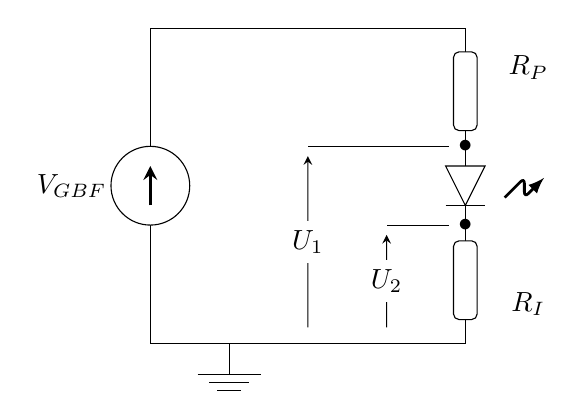
\begin{tikzpicture}
    \draw(0,-2)--(0,2)--(4,2)--(4,-2)--cycle;
    \draw[fill=white] (0,0) circle (0.5cm);
    \draw [>=stealth, ->, very thick] (0,-0.25)--(0,0.25);
    \node at (-1,0) {$V_{\text{GBF}}$};
    \node[draw, fill=white, minimum width=0.3cm, minimum height=1cm, rounded corners =2pt] at (4,1.2) {};
    \node [xshift=0.8cm] at (4,1.5) {$R_{P}$};
    \draw(1,-2)--++(0,-0.4); \draw(0.6,-2.4)--++(0.8,0); \draw (0.75,-2.5)--++(0.5,0);\draw (0.85,-2.6)--++(0.3,0); 
     \node[draw, fill=white, minimum width=0.3cm, minimum height=1cm, rounded corners =2pt] at (4,-1.2) {};
    \node [xshift=0.8cm] at (4,-1.5) {$R_I$};
            \begin{scope}[xshift=3.75cm, yshift=0.25 cm]%LED
            \draw[fill=white] (0,0)--++(0.5,0)--++(-0.25,-0.5)--cycle;
            \draw (0,-0.5)--++(0.5,0); %node[above right, yshift=0.5cm]{LED};
            \draw[->,>=latex,rounded corners=2pt, line width=1pt] (0.75,-0.4) --++ (0.25,0.25)--++(0,-0.25)--++(0.25,0.25);
            \node (A1) at (0.25,0) {};
            \node (K1) at (0.25,-0.5) {};
            \end{scope}        
            
           \node[yshift=0.25 cm]  (CH1) at (A1){$\bullet$};
            \node[yshift=-0.25 cm] (CH2)   at (K1){$\bullet$};
           \draw (CH1) --++(-2,0) node (VCH1) {};
           \draw (CH2) --++(-1,0)node (VCH2) {};
%            
           \draw [<-, >=stealth] (VCH1) -- (2,-1.8) node [midway, fill=white] {$U_{1}$};
            \draw [<-, >=stealth] (VCH2) -- (3,-1.8) node [midway, fill=white] {$U_{2}$};
\end{tikzpicture}

\end{multicols}


\subsubsection*{Méthode de mesure}

On applique un signal dont l'amplitude varie dans le temps à l'aide du GBF : un signal triangulaire par exemple à une fréquence de quelques Hertz. \textit{On s'assurera que l'amplitude du signal fourni par le GBF est inférieure aux limitations des composants du montage.}

En mesurant à l'oscilloscope les tensions $U_1$ sur une voie et $U_2$ sur l'autre voie, on accède à une image de la tension aux bornes du dipôle ($U_1 – U_2$, assimilable à $U_1$ si $U_2$ est faible pour toutes les valeurs de $i$) et à une image du courant traversant $R_I$ ($U_2$).

En traçant alors $U_2$ en fonction de $U_1$ (mode XY de l'oscilloscope), l'allure de la caractéristique statique du dipôle s'affiche alors.

\newpage
\pagestyle{empty}

\begin{minipage}[c]{.25\linewidth}
	
\includegraphics[width=4cm]{images/Logo-LEnsE.png}
\end{minipage} \hfill
\begin{minipage}[c]{.4\linewidth}

\begin{center}
\vspace{0.3cm}
{\Large \textsc{Opto-Electronique}}

\medskip

\textbf{\Large Ressources}

\end{center}
\end{minipage}\hfill

\vspace{0.5cm}

\noindent \rule{\linewidth}{1pt}
\section{Tracer la réponse indicielle d'un système linéaire}
\label{ressource:RepIndic}


%%%%%%%%%%%%%%%%%%%%

La réponse indicielle fournit des informations essentielles sur les \textbf{caractéristiques dynamiques} d'un système. Elle permet d'analyser le comportement transitoire et le comportement à l'état stable d'un système. Par exemple, on peut observer le temps de montée, le temps de stabilisation, le dépassement (ordre supérieur à 2), et l'erreur en régime permanent.

Elle est aussi appelée \textbf{réponse à un échelon} unitaire. Elle correspond à la sortie d'un système lorsqu'un signal de type échelon est appliqué en entrée. Un \textbf{échelon unitaire} est une fonction qui passe de 0 à 1 à un instant donné, généralement considéré à $t = 0$. 

La figure~\ref{fig:ordre2} est une capture d'écran d'oscilloscope représentant la réponse indicielle d'un système passe-bas du second ordre. 

\begin{figure}[h!]
    \centering
	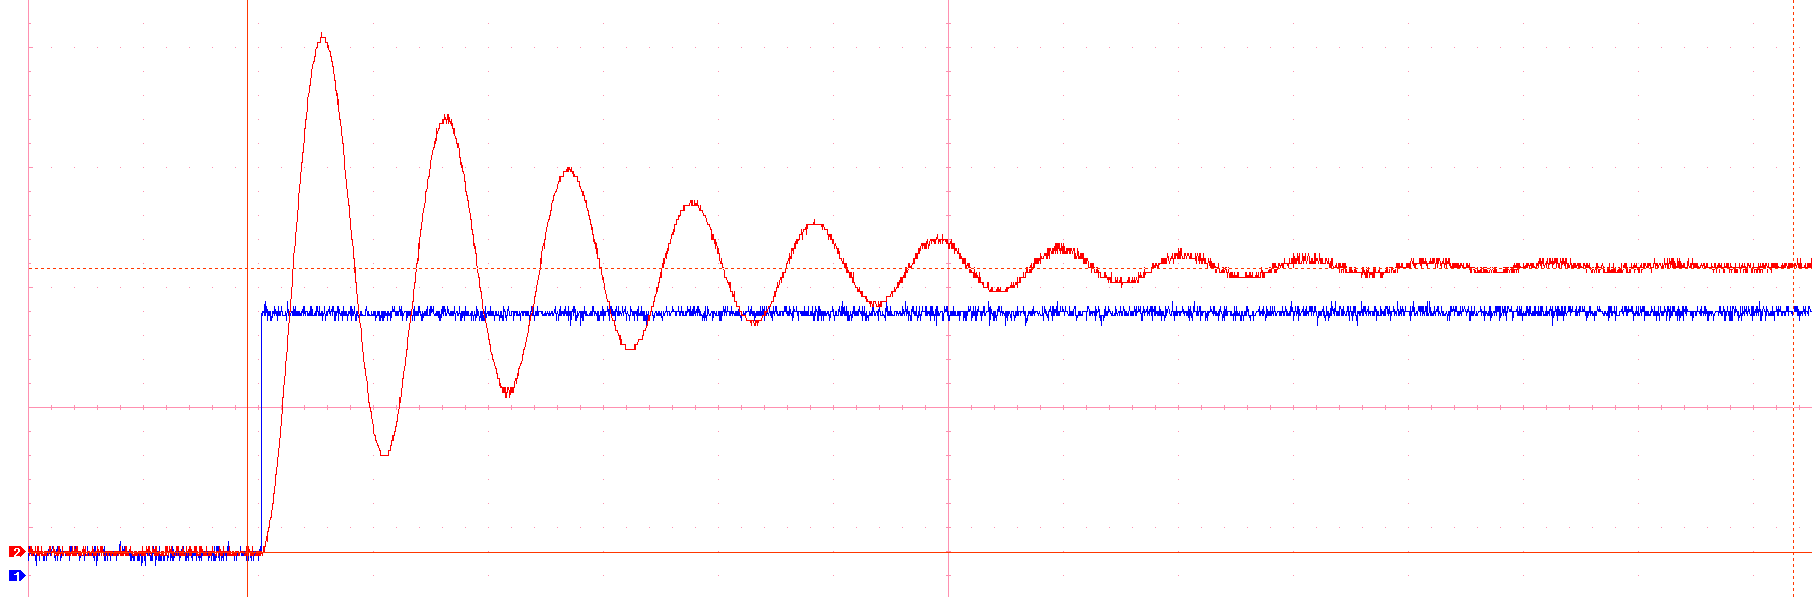
\includegraphics[width=0.9\textwidth]{images/ri_ordre2.png}
	
    \caption{Capture d'écran d'oscilloscope d'un échelon de tension $V_E$ (en bleu) appliqué à un système de type passe-bas d'ordre 2 avec résonance. La tension de sortie $V_S$ (en rouge) représente la réponse indicielle de ce système. Le calibre vertical est de 1V/carreau pour $V_E$ et de 2V/carreau pour $V_S$. L'échelle horizontale est de 1ms/carreau.}
    \label{fig:ordre2}
\end{figure}


%%%%%%%%%%%%%%%%%%%%%%%%%%%%%%%%%%
\subsection{Méthode de mesure}

Pour mesurer la réponse à un échelon, il faut appliquer un signal rectangulaire lent, laissant le temps au système de revenir à un état stable.

\textit{Il faut également faire en sorte que l'amplitude du signal d'entrée n'entraine pas de saturation du signal de sortie (cas des systèmes actifs intégrant des amplificateurs linéaires par exemple).}

\medskip

On visualise ensuite le signal d'entrée à l'oscilloscope, qui nous servira de signal de déclenchement (front montant), et le signal de sortie du système à analyser.



\newpage
%%%%%%%%%%%%%%%%%%%%%%%%%%%%%%%%%%
\subsection{Mesure du gain}

Un élément caractérisant un système linéaire est son gain dans la bande passante. On peut mesurer à l'aide des curseurs l'amplitude de l'échelon sur l'entrée $\Delta{}V_e$ et l'écart de tension entre les deux états stables de la sortie $\Delta{}V_s$. Le gain du système dans la bande-passante vaut alors $G = \Delta{}V_s / \Delta{}V_e$.

\medskip

La figure~\ref{fig:ordre1_gain} montre une capture d'écran de l'acquisition à l'oscilloscope d'une réponse indicielle d'un système passe-bas du premier ordre.

Les valeurs de $\Delta{}V_e$ et $\Delta{}V_s$ peuvent être mesurées aux endroits indiqués par les flèches (cas d'un passe-bas).


\begin{figure}[h!]
    \centering
	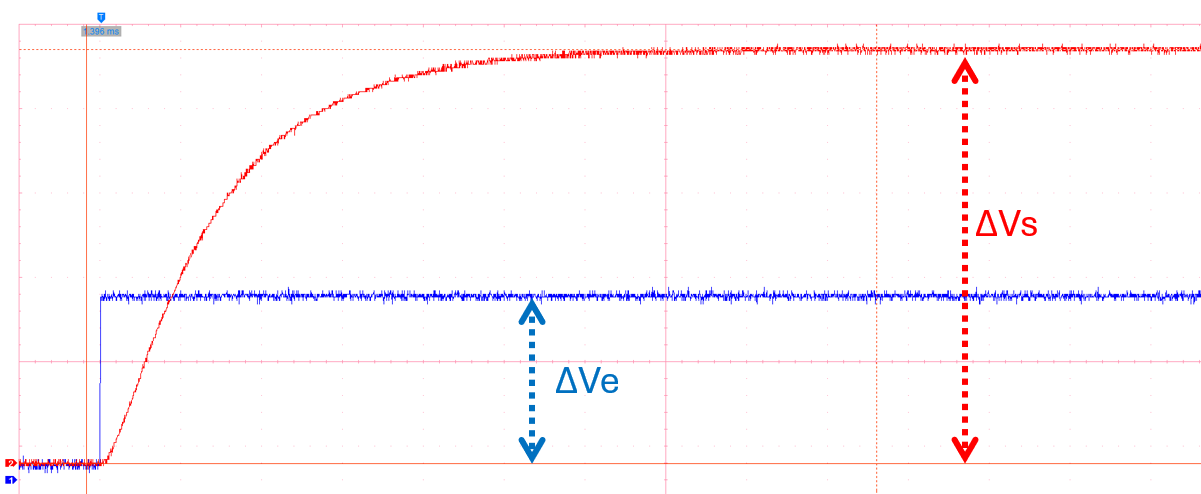
\includegraphics[width=0.5\textwidth]{images/ri_ordre1_out.png}
	
	%Cas d'un système passe-bas d'ordre 1 - mesure de la tension de sortie.
	
    \caption{Capture d'écran d'oscilloscope d'un échelon de tension $V_E$ (en bleu) appliqué à un système de type passe-bas d'ordre 1. La tension de sortie $V_S$ (en rouge) représente la réponse indicielle de ce système. Le calibre vertical est de 1V/carreau pour $V_E$ et de 1V/carreau pour $V_S$. L'échelle horizontale est de 1ms/carreau.}
    \label{fig:ordre1_gain}
\end{figure}



%%%%%%%%%%%%%%%%%%%%%%%%%%%%%%%%%%
\subsection{Mesure du temps de réponse}

Une autre information importante, en lien avec la bande-passante du système, est son temps de réponse. 

Dans le cas des systèmes d'ordre 1, le temps que met le système à atteindre 63\% de la valeur finale correspond à $\tau$, la constante de temps du système.

Dans la majorité des cas, on chercher à mesurer le temps que met le système à atteindre 95\% de sa valeur finale.

\medskip

La figure~\ref{fig:ordre1_response} montre une capture d'écran de l'acquisition à l'oscilloscope d'une réponse indicielle d'un système passe-bas du premier ordre.

Les positions de relevé de mesures des différents temps de réponse (63\% de la valeur finale pour un système d'ordre 1 ou 95\% de la valeur finale dans la majorité des cas) sont indiquées également sur cette figure.

\begin{figure}[h!]
    \centering
	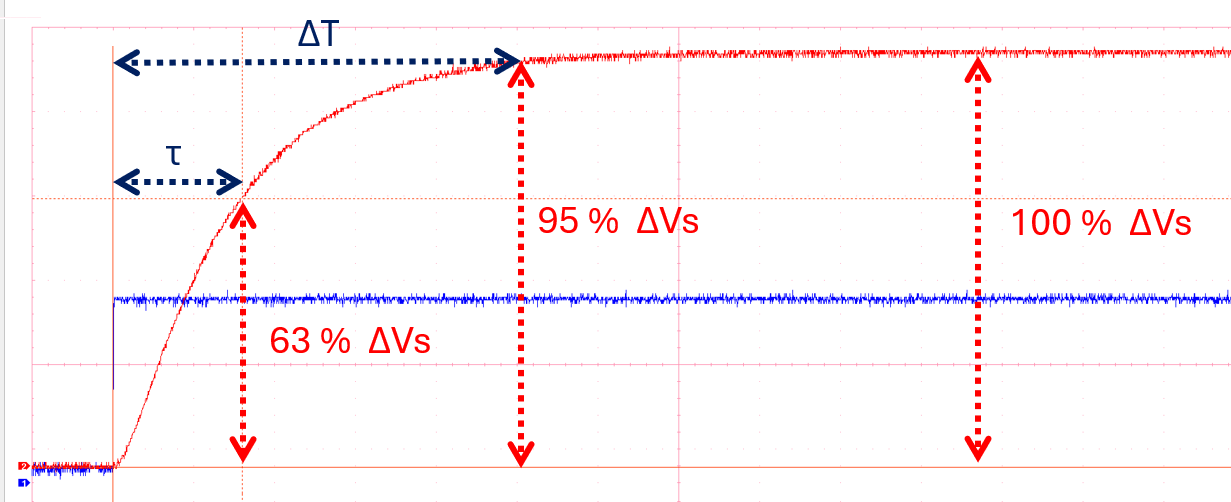
\includegraphics[width=0.6\textwidth]{images/ri_ordre1_out_63.png}
	
	%Cas d'un système passe-bas d'ordre 1 - mesures de la constante de temps et du temps de réponse à 95\%.
	
	    \caption{Capture d'écran d'oscilloscope d'un échelon de tension $V_E$ (en bleu) appliqué à un système de type passe-bas d'ordre 1. Mesures de la constante de temps et du temps de réponse à 95\%. La tension de sortie $V_S$ (en rouge) représente la réponse indicielle de ce système. Le calibre vertical est de 1V/carreau pour $V_E$ et de 2V/carreau pour $V_S$. L'échelle horizontale est de 1ms/carreau.}
    \label{fig:ordre1_response}
\end{figure}

\newpage
%%%%%%%%%%%%%%%%%%%%%%%%%%%%%%%%%%
\subsection{Autres mesures}

Il peut être intéressant de relever les valeurs des surtensions lors des \textbf{dépassements} (cas de systèmes d'ordre supérieur à 2). On peut par exemple, à l'aide des curseurs, mesurer le dépassement $D1$ (en lien avec le facteur de qualité d'un système du second ordre).

La période des oscillations $T$ peut également être mesurée (en lien avec la pulsation propre du système).

\medskip

La figure~\ref{fig:ordre2_dep} est une capture d'écran d'oscilloscope suite à l'acquisition d'une réponse indicielle d'un système passe-bas du second ordre. La méthode de mesure du premier dépassement ainsi que de la période des pseudo-oscillations est représentée.

\begin{figure}[h!]
    \centering
	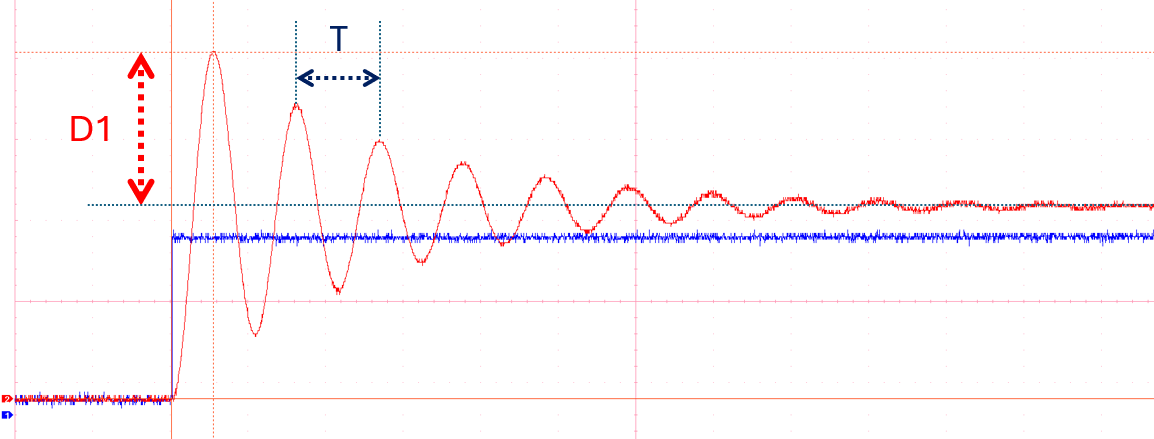
\includegraphics[width=0.6\textwidth]{images/ri_ordre2_bas_out_d1.png}
	
	%Cas d'un système passe-bas d'ordre 2 avec résonance - mesure de D1.    
	\caption{Capture d'écran d'oscilloscope d'un échelon de tension $V_E$ (en bleu) appliqué à un système de type passe-bas d'ordre 2 avec résonance. La tension de sortie $V_S$ (en rouge) représente la réponse indicielle de ce système. Le calibre vertical est de 1V/carreau pour $V_E$ et de 2V/carreau pour $V_S$. L'échelle horizontale est de 1ms/carreau.}
    \label{fig:ordre2_dep}
\end{figure}



%%%%%%%%%%%%%%%%%%%%%%%%%%%%%%%%%%
\subsection{Lien avec la réponse impulsionnelle et la réponse en fréquence}

La réponse indicielle est liée à la réponse impulsionnelle $h(t)$ d'un système par la relation suivante :

$$u_S(t) = \int_{0}^t h(x)dx$$

Cela signifie que la réponse indicielle est l'intégrale de la réponse impulsionnelle.

On rappelle également que la réponse en fréquence, que l'on peut modéliser par la fonction de transfert d'un circuit en fonction de la fréquence $H(j\omega)$ est la transformée de Fourier de la réponse impulsionnelle $h(t)$.

\newpage
\pagestyle{empty}

\begin{minipage}[c]{.25\linewidth}
	
\includegraphics[width=4cm]{images/Logo-LEnsE.png}
\end{minipage} \hfill
\begin{minipage}[c]{.4\linewidth}

\begin{center}
\vspace{0.3cm}
{\Large \textsc{Opto-Electronique}}

\medskip

\textbf{\Large Ressources}

\end{center}
\end{minipage}\hfill

\vspace{0.5cm}

\noindent \rule{\linewidth}{1pt}
\section{Tracer la réponse en fréquence d'un système linéaire}
\label{ressource:RepFreq}


%%%%%%%%%%%%%%%%%%%%%%%%%%%%%%%%%%%%%%%%%%%%%%%%%%%%%%%%%%%%%%%%%%%%%%%%%%%%%%%%
%%%%%

La réponse en fréquence décrit la manière dont \textbf{un système réagit à différentes fréquences d'entrée}. Elle indique comment l'amplitude et la phase d'un signal sont modifiées lorsqu'il passe à travers un système ou un circuit, en fonction de la fréquence du signal.

Cette étude traduit le \textbf{comportement harmonique} d'un circuit, c'est à dire sa réponse à une excitation (en tension) sinusoïdale.

Cette fonction n'est définie que dans le cas de circuits linéaires. La tension de sortie est dans ce cas sinusoïdale et de même fréquence que le signal d'entrée.

\subsection{Objectif}

Obtenir l'allure de la \textbf{courbe du gain} et éventuellement de celle \textbf{du déphasage} apportés par le circuit en fonction de la fréquence du signal sinusoïdal placé en entrée.

Le \textbf{diagramme de Bode} est une manière spécifique de représenter la réponse en fréquence. Il s'agit d'une \textbf{représentation graphique} qui se compose de deux parties distinctes :

\begin{itemize}
	\item diagramme de Bode en gain (gain en $\operatorname{dB}$),
	\item diagramme de Bode en phase.
\end{itemize}

\bigskip

La courbe est souvent tracée avec une \textbf{échelle logarithmique} en fréquence. 

\subsection{Intérêt du passage en décibels (dB)}

Lorsqu'on cascade plusieurs systèmes entre eux, leurs fonctions de transfert se multiplient. Il n'est alors pas simple de pouvoir comparer \textbf{graphiquement} les systèmes à plusieurs étages facilement.

$$A = \prod_{k=1}^{n} A_k $$

En passant par une échelle logarithmique (en décibels par exemple), on transforme ce produit en une somme. Ainsi il sera plus simple de cumuler les effets d'une mise en cascade de systèmes linéaires et de voir le comportement global en additionnant les comportements de chacun des étages.

$$G_{dB} = \log(A) = \log(\prod_{k=1}^{n} A_k) = \sum_{k=1}^{n} \log(A_k) $$

\newpage
\subsection{Protocole d'étude}

\begin{itemize}
	\item Régler un \textbf{générateur de fonction} (ou GBF) pour avoir un \textbf{signal sinusoïdal} à sa sortie, avec une amplitude compatible avec les limites du circuit à tester.
	\item Relier le générateur de fonction à la fois à l'entrée du circuit et à une des entrées de l'oscilloscope.
	\item Relier la tension de sortie à une deuxième voie de l'oscilloscope.
	\item \textbf{S'assurer que le signal de sortie est bien sinusoïdal} avant d'aller plus loin. Dans le cas contraire, le système ne fonctionne pas de manière linéaire (amplitude trop élevée en entrée par exemple qui entraine une saturation en sortie...)
\end{itemize}


\section{Procédure classique}

Un premier balayage rapide en fréquence permet de \textbf{repérer les gammes de fréquences d'intérêt}.

Une analyse du \textbf{comportement du circuit pour les valeurs extrêmes de fréquences} (sur la phase et l'amplitude) apporte les informations sur le comportement asymptotique de la réponse en fréquence. Ce sont les \textbf{2 premiers points de mesure}.

\textbf{3 à 5 mesures supplémentaires} sont ensuite suffisantes :
\begin{itemize}
	\item l'une à la fréquence caractéristique du circuit, qui peut être : 
	\begin{itemize}
		\item la fréquence centrale d'un circuit passe-bande, 
		\item la bande passante à $-3\operatorname{dB}$ pour un circuit passe-bas ou passe-haut,
		\item la fréquence d'un déphasage particulier (en général la fréquence pour laquelle le déphasage apporté est égal à la moitié du déphasage maximal que le circuit peut apporter )
	\end{itemize}
	\item les autres de part et d'autres de cette fréquence caractéristique, à une octave au dessous (à la fréquence moitié) et une octave au dessus ( à la fréquence double)
\end{itemize}

\medskip

La figure~\ref{fig:rf_mesure} montre une capture d'écran d'oscilloscope d'un signal sinusoïdal $V_E$ appliqué à un système linéaire et sa sortie $V_S$. La méthode de mesure du gain du montage et du déphasage pour une fréquence particulière est représentée sur cette figure également.

\begin{figure}[h!]
    \centering
	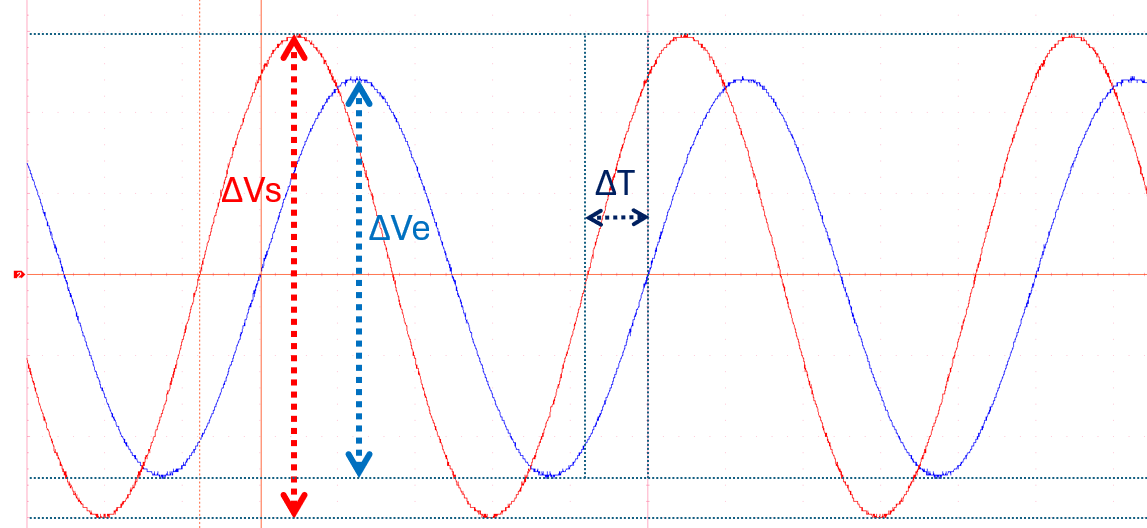
\includegraphics[width=0.8\textwidth]{images/rf_bode.png}
	
    \caption{Capture d'écran d'oscilloscope d'un signal sinusoïdal $V_E$ (en bleu) appliqué à un système linéaire et sa sortie $V_S$ (en rouge). Le calibre vertical est de 200mV/carreau pour $V_E$ et pour $V_S$. L'échelle horizontale est de 2ms/carreau.}
    \label{fig:rf_mesure}
\end{figure}

\newpage
\subsection{Mesure du gain du circuit}

Il existe \textbf{deux solutions pour déterminer la valeur du gain} :

\begin{itemize}
	\item Utiliser les mesures automatiques de l'oscilloscope, pour relever l'amplitude du signal d'entrée ($\Delta{}V_e$) et du signal de sortie ($\Delta{}V_s$), et utiliser un logiciel pour convertir le gain en $\operatorname{dB}$
	\item Utiliser le multimètre en dB-mètre (voir documentation annexe des instruments de mesure).
\end{itemize}

\medskip

On rappelle que le gain en décibel est égal à :

$$G_{dB} = 20 \cdot \log(A)$$

où $A = \frac{\Delta{}V_s}{\Delta{}V_e}$ est le gain du système.

\subsection{Mesure du déphasage}

Certains oscilloscopes proposent des mesures automatiques du déphasage. En leur absence, une mesure aux curseurs du décalage temporel $\Delta{}T$ entre les deux tensions (entrée et sortie) permet de remonter au déphasage $\Delta{}\phi$ par la formule :

$$\Delta{}\phi = +/- \frac{\Delta{}T}{T} \cdot 2\pi$$

où T est la période du signal.

Il est important de déterminer lequel des deux signaux est en avance sur l'autre, afin de donner un signe au déphasage apporté par le circuit. Si la tension de sortie est en retard sur la tension d'entrée, le déphasage est négatif.

\newpage
\section{Allure rapide}

Il existe également une \textbf{méthode automatique} pour obtenir l'allure de la réponse en fréquence du système, selon le modèle de GBF que vous possédez.

En effet, certains d'entre eux sont capables de réaliser automatiquement un balayage en fréquence.

Pour les GBF \textbf{\texttt{Agilent}} (des salles de TP d'électronique, par exemple), il faut utiliser au préalable sélectionner un \textbf{signal sinusoïdal}, de n'importe quelle fréquence mais d'amplitude et de valeur moyenne (offset) compatible avec le système à étudier (si ALI/AOP, vérifiez que le signal de sortie ne sature pas, par exemple).

Puis sélectionner ensuite le menu \textbf{Sweep} du GBF. Se référer ensuite à la documentation du GBF fournie sur vos paillasses pour les réglages (voir aussi figure~\ref{fig:gbf_sweep}).

\begin{figure}[h!]
    \centering
	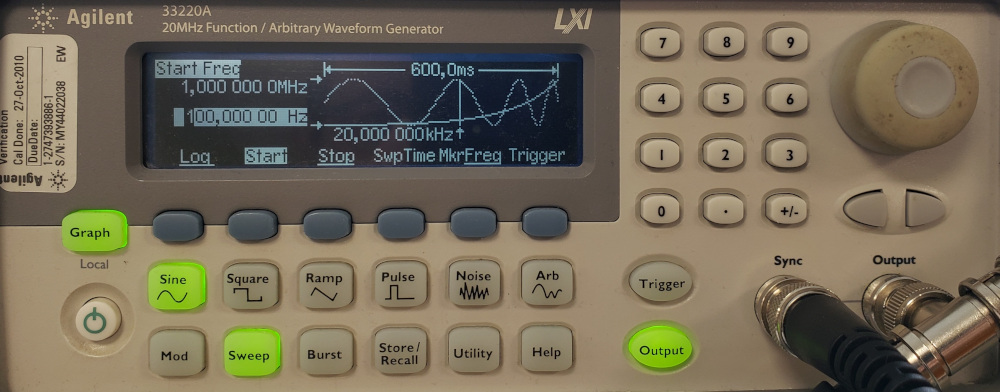
\includegraphics[width=0.6\textwidth]{images/gbf_sweep.jpg}
	
    \caption{Photographie d'un générateur de fonction Agilent 33220A en mode \textit{sweep} (balayage).}
    \label{fig:gbf_sweep}
\end{figure}


Il est ensuite possible de synchroniser l'oscilloscope avec le GBF en utilisant la sortie \textbf{Sync}, qui fournit un signal rectangulaire de même période que le balayage, connectée à l'une des entrées de l'oscilloscope (EXT si on ne souhaite que synchroniser) et en réglant les paramètres du déclenchement de l'oscilloscope.

\begin{figure}[h!]
    \centering
	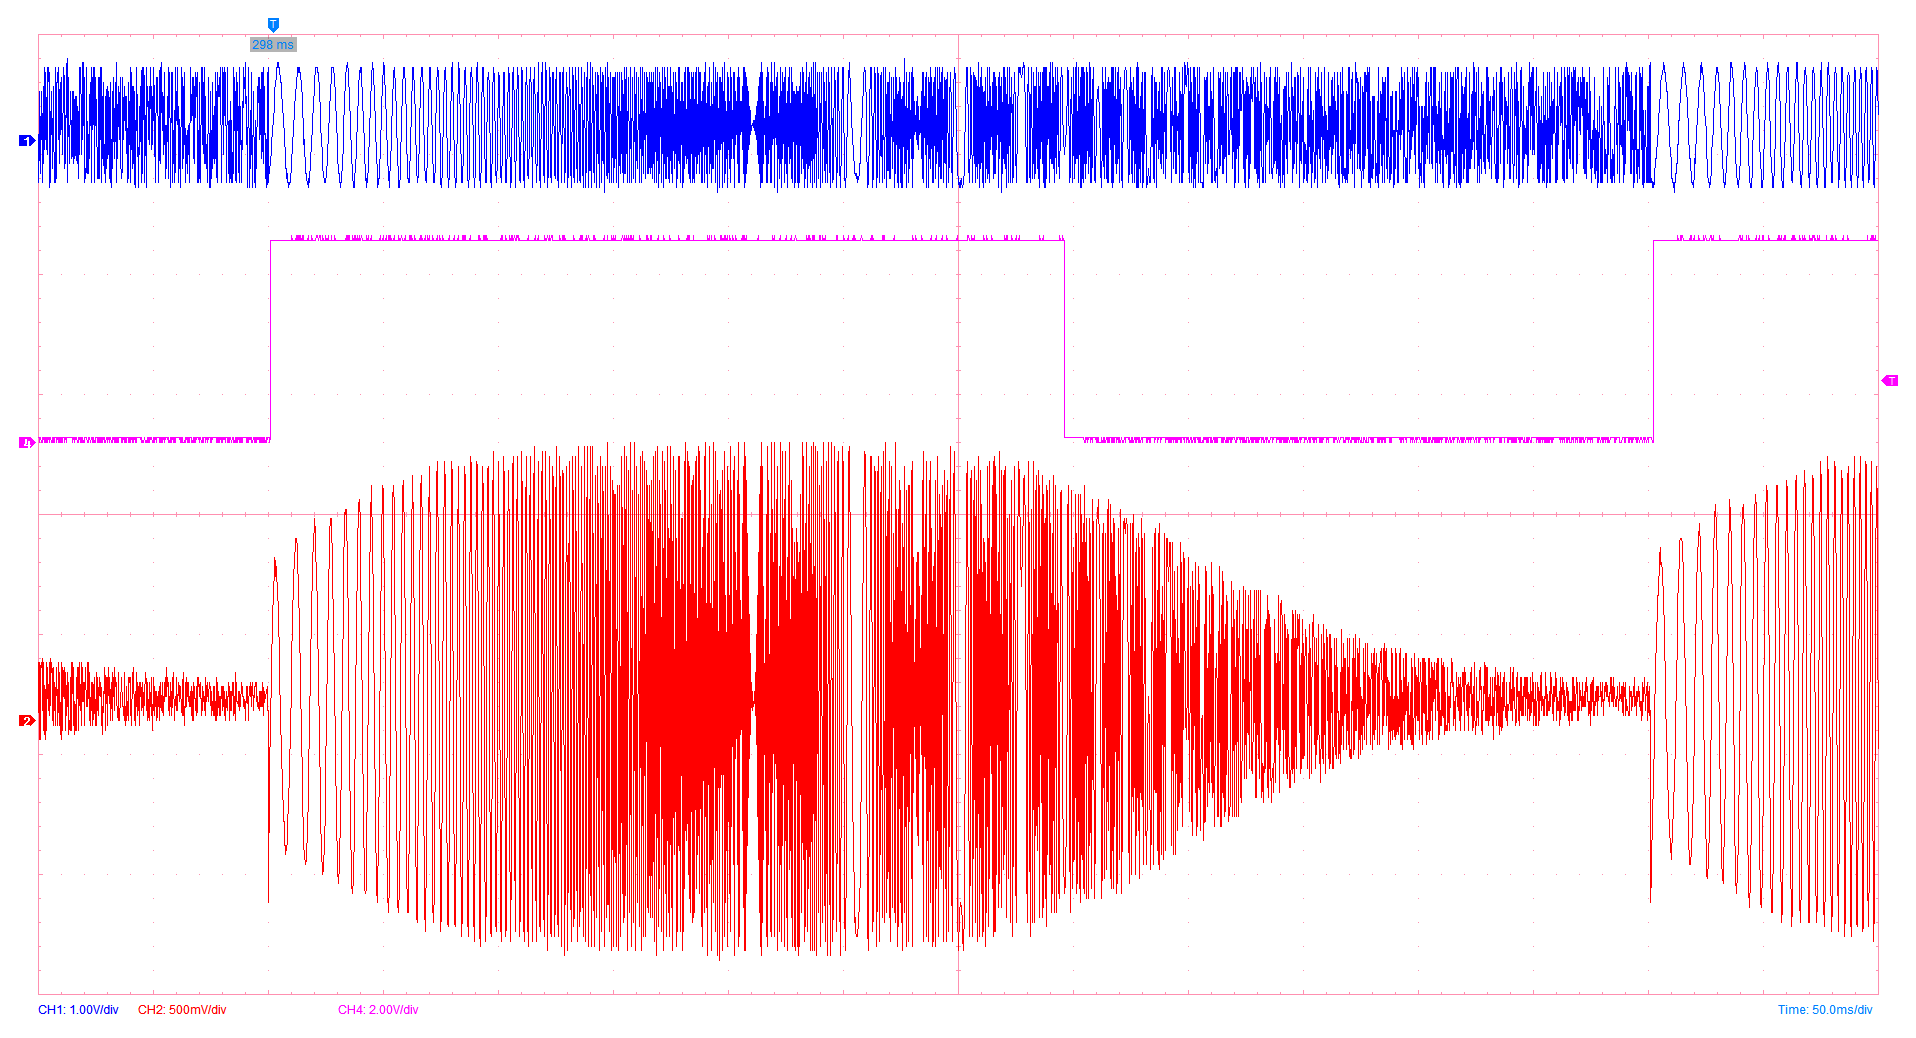
\includegraphics[width=0.7\textwidth]{images/gbf_sweep_sync.png}
	
	%Cas d'un passe-bande - en haut signal d'entrée (amplitude constante), au centre signal de synchronisation (avec marqueur en fréquence - retour à l'état bas) et en bas signal de sortie.

	
    \caption{Capture d'écran d'oscilloscope d'un balayage en fréquence $V_E$ (en bleu) appliqué à un système linéaire et sa sortie $V_S$ (en rouge) - cas d'un passe-bande. En haut signal d'entrée $V_E$ (amplitude constante), au centre signal de synchronisation (avec marqueur en fréquence - retour à l'état bas) et en bas signal de sortie $V_S$. Le calibre vertical est de 1V/carreau pour $V_E$ et de 200mV/carreau pour $V_S$. L'échelle horizontale est de 50ms/carreau.}
    \label{fig:rf_sweep}
\end{figure}

\newpage
\section{Quelques rappels}
%%%%%%%%%%%%%%%%%%%%%%%%%%%%%%%%%%
\subsection{Déphasage}

En régime harmonique (à même fréquence), deux ondes sinusoïdales peuvent avoir des phases initiales différentes.

Soient $u_1(t) = A_1 \cdot sin(2\pi f t + \varphi_1)$ et $u_2(t) = A_2 \cdot sin(2\pi f t + \varphi_2)$, le déphasage de l'une par rapport à l'autre à l'instant $t$ vaut : $\Delta\varphi = (2\pi f t + \varphi_2) - (2\pi f t + \varphi_1) = \varphi_2 - \varphi_1$

\medskip

Si $\Delta\varphi$ est positif, l'onde 2 est en avance de phase par rapport à l'onde 1. Sinon, l'onde 2 est en retard de phase par rapport à l'onde 1.

%%%%%%%%%%%%%%%%%%%%%%%%%%%%%%%%%%
\subsection{Phase et ordre d'un filtre}

Lorsqu'on étudie des systèmes linéaires de type filtre, il est intéressant de relever le déphasage entre le signal de sortie et le signal d'entrée pour différents points remarquables :

\begin{itemize}
	\item à la fréquence caractéristique du système, le déphasage est égal à $k\cdot \pi/4$ où $k$ est un entier correspondant à l'ordre du filtre
	\item loin de cette fréquence caractéristique (au moins une décade avant et après), pour vérifier le caractère inverseur d'un système par exemple.
\end{itemize}


\newpage
\pagestyle{empty}

\begin{minipage}[c]{.25\linewidth}
	
\includegraphics[width=4cm]{images/Logo-LEnsE.png}
\end{minipage} \hfill
\begin{minipage}[c]{.4\linewidth}

\begin{center}
\vspace{0.3cm}
{\Large \textsc{Opto-Electronique}}

\medskip

\textbf{\Large Ressources}

\end{center}
\end{minipage}\hfill

\vspace{0.5cm}

\noindent \rule{\linewidth}{1pt}
\section{Mesurer la bande-passante d'un système linéaire}
\label{ressource:BandePassante}


%%%%%%%%%%%%%%%%%%%%%%%%%%%%%%%%%%%%%%%%%%%%%%%%%%%%%%%%%%%%%%%%%%%%%%%%%%%%%%%%
%%%%%

La \textbf{bande-passante} est un \textbf{paramètre crucial} pour évaluer et concevoir des systèmes électroniques, des filtres, des amplificateurs et des circuits de communication. Elle est définie comme l'\textbf{intervalle de fréquences} pour lequel le système peut \textbf{transmettre des signaux avec une atténuation minimale}.

\medskip

Pour les systèmes linéaires et les filtres, la bande-passante est souvent mesurée entre les points où la puissance du signal de sortie est \textbf{réduite de $3\operatorname{dB}$} par rapport à la puissance du signal de sortie dans la bande-passante (voir figure~\ref{fig:rf_bp}).

\begin{figure}[h!]
    \centering
	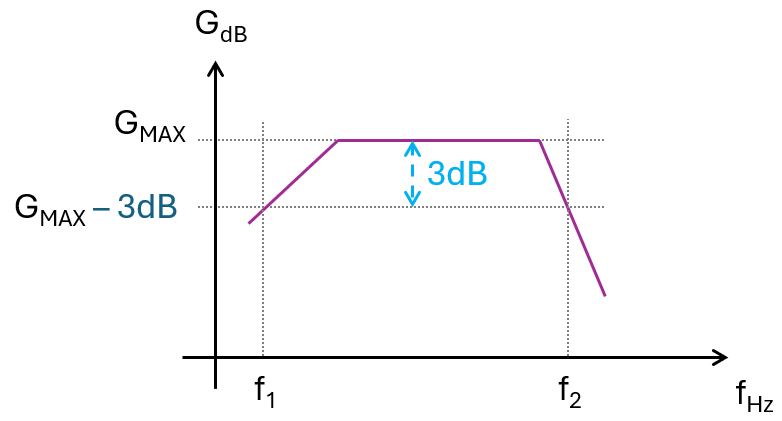
\includegraphics[width=0.6\textwidth]{images/bande_passante.png}
	
    \caption{Schéma de principe de la mesure de la bande-passante d'un système linéaire. Allure de la courbe de réponse en fréquence. La bande-passante de ce système s'étend de $f_1$ à $f_2$. Cela correspond donc à l'intervalle $\left[ f_1, f_2 \right]$.}
    \label{fig:rf_bp}
\end{figure}




\subsection{Mesure graphique}

A partir de la \textbf{réponse en fréquence}, il est possible de mesurer graphiquement la bande passante en cherchant le gain maximal du système et en regardant l'intersection des points passant par ce gain maximal réduit de $3\operatorname{dB}$ et l'axe des fréquences.


\subsection{Mesure expérimentale}

Cette réduction de $3\operatorname{dB}$ peut aussi être interprétée comme une \textbf{diminution de l'amplitude du signal d'un facteur} $\sqrt{2}$ par rapport à l'amplitude du signal de sortie dans la bande-passante (\textit{en supposant que le signal d'entrée reste constant en amplitude quelque soit sa fréquence}).

Il est donc possible de mesurer le gain maximal (à l'aide d'un oscilloscope ou d'un multimètre) en cherchant une fréquence telle que l'amplitude du signal de sortie sur celle d'entrée est maximale, en mesurant ces deux valeurs.

On cherche ensuite les amplitudes telles que le gain maximal est divisé par $\sqrt{2}$ et on relève les fréquences associées. Ces fréquences correspondent à la bande-passante.

\cleardoublepage
\ifodd\value{page}\else
  \hbox{}\newpage
\fi
%% Fiches 

\titleformat{\section}
  {\null}{}{0pt}{}
  
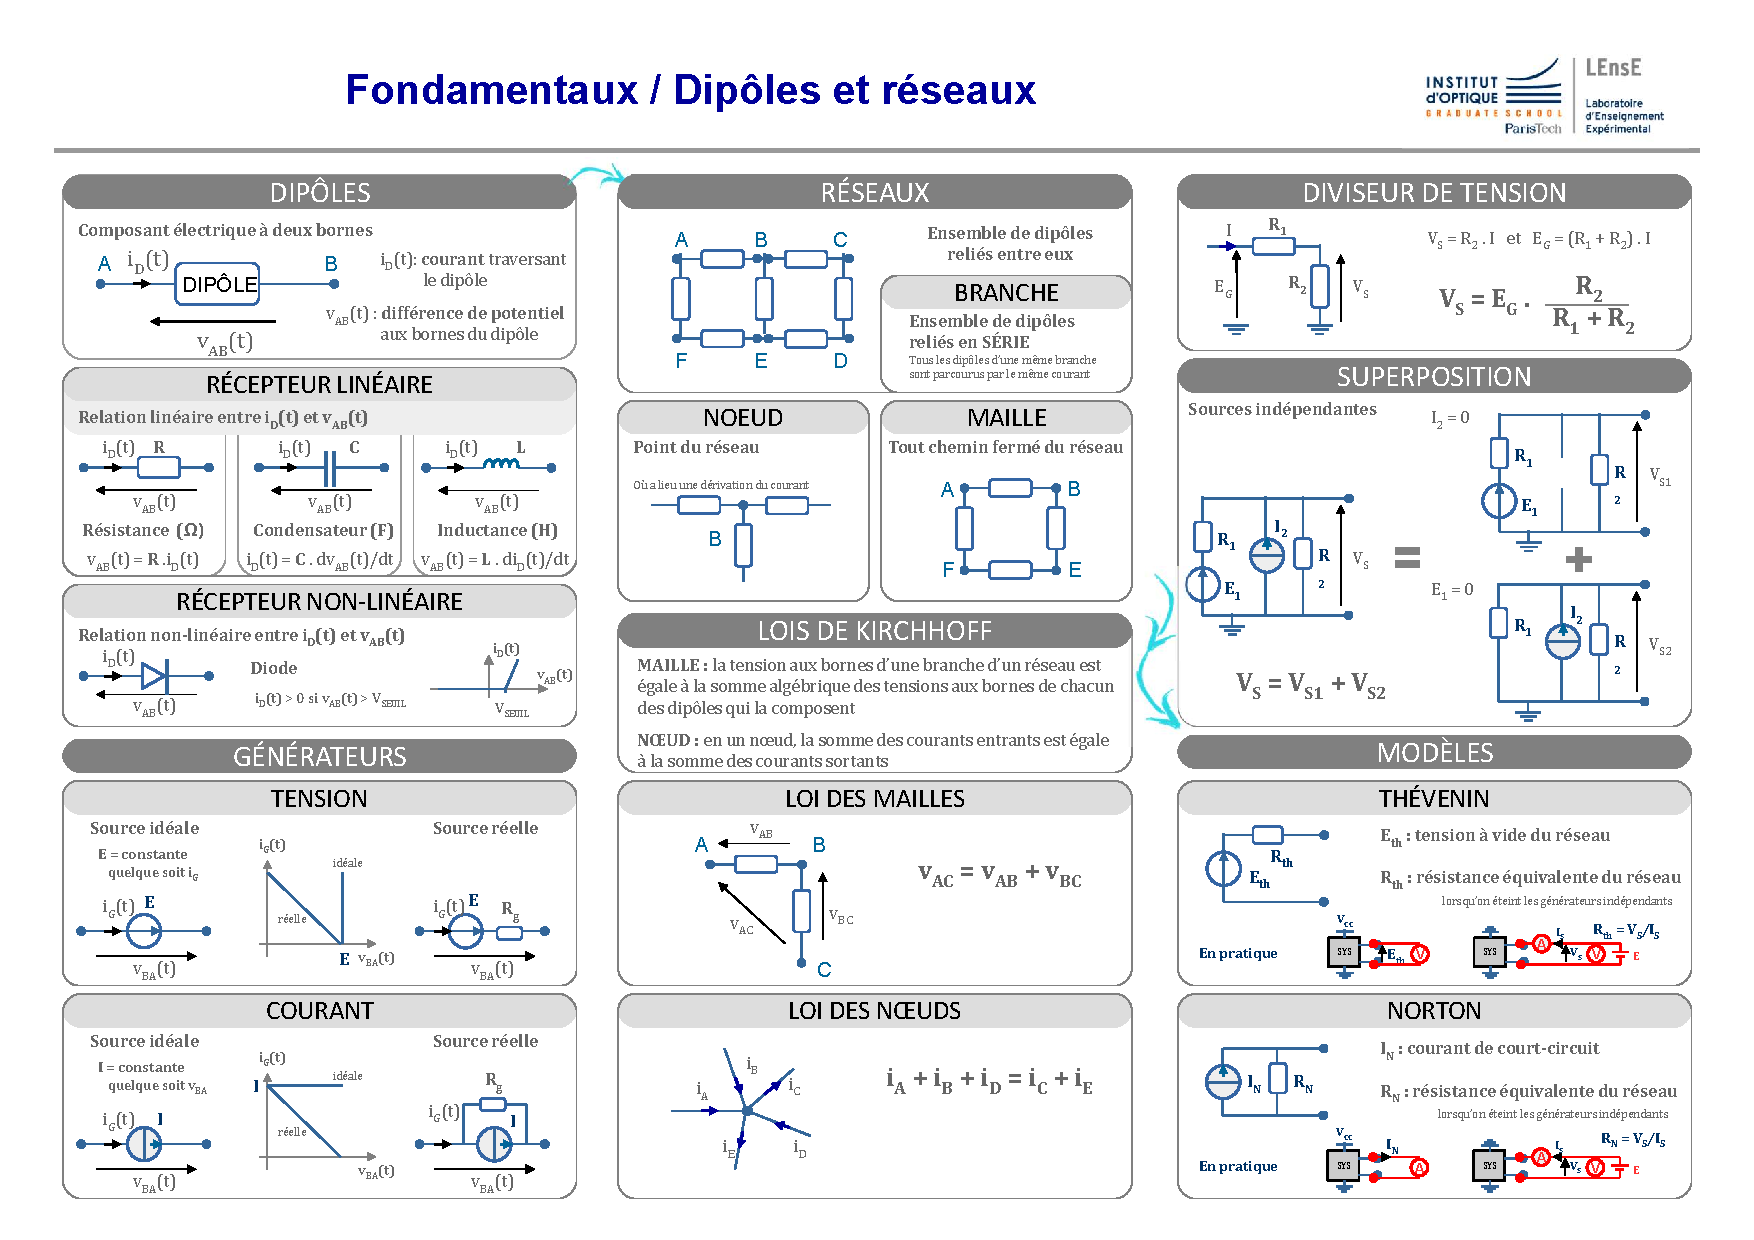
\includepdf[pages=-, landscape=true, pagecommand={\section{\texorpdfstring{\hspace{-1em}}{Fiche Bases}}}\label{fiche:Bases1}]{../../../Fiches/Fiche_Bases1.pdf}


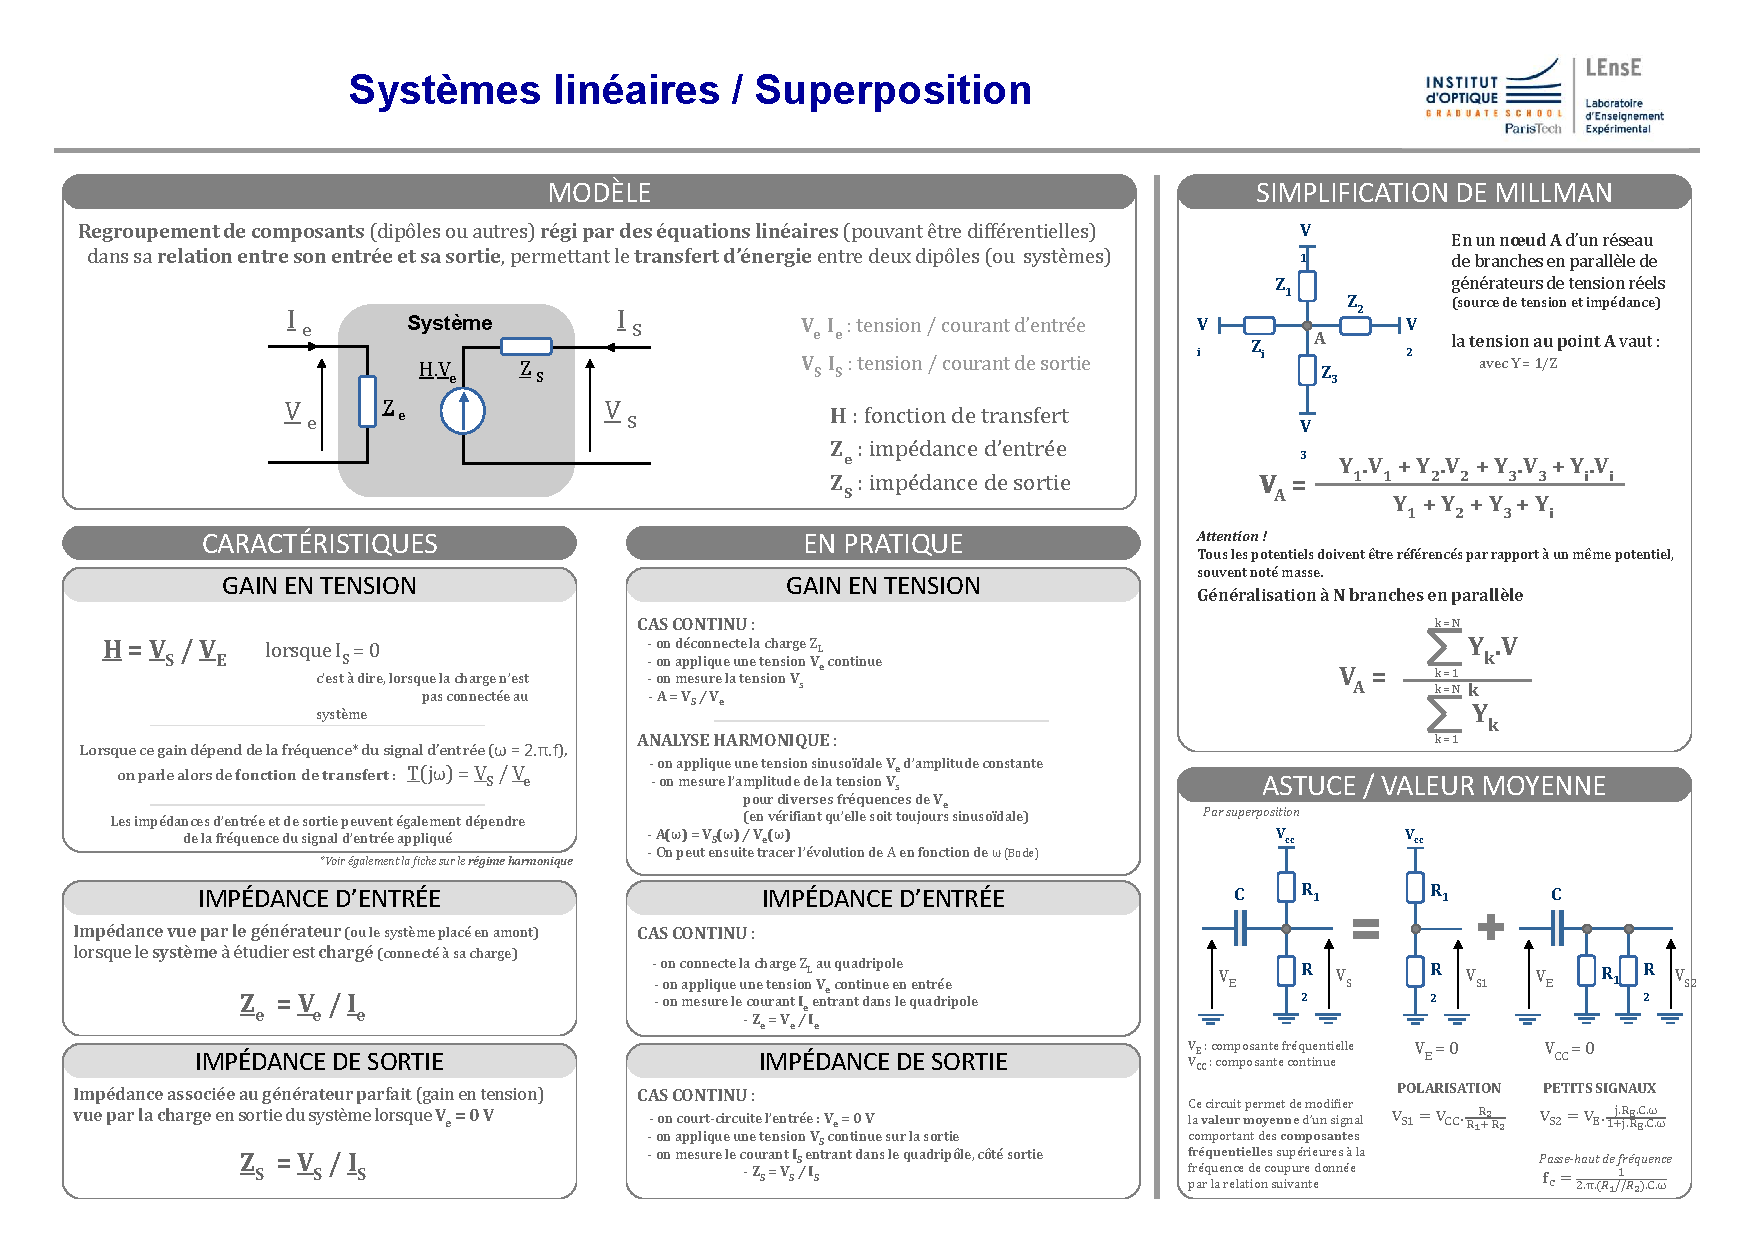
\includepdf[pages=-, landscape=true, pagecommand={\section{\texorpdfstring{\hspace{-1em}}{Fiche Superposition}}}\label{fiche:Bases2}]{../../../Fiches/Fiche_Bases2.pdf}

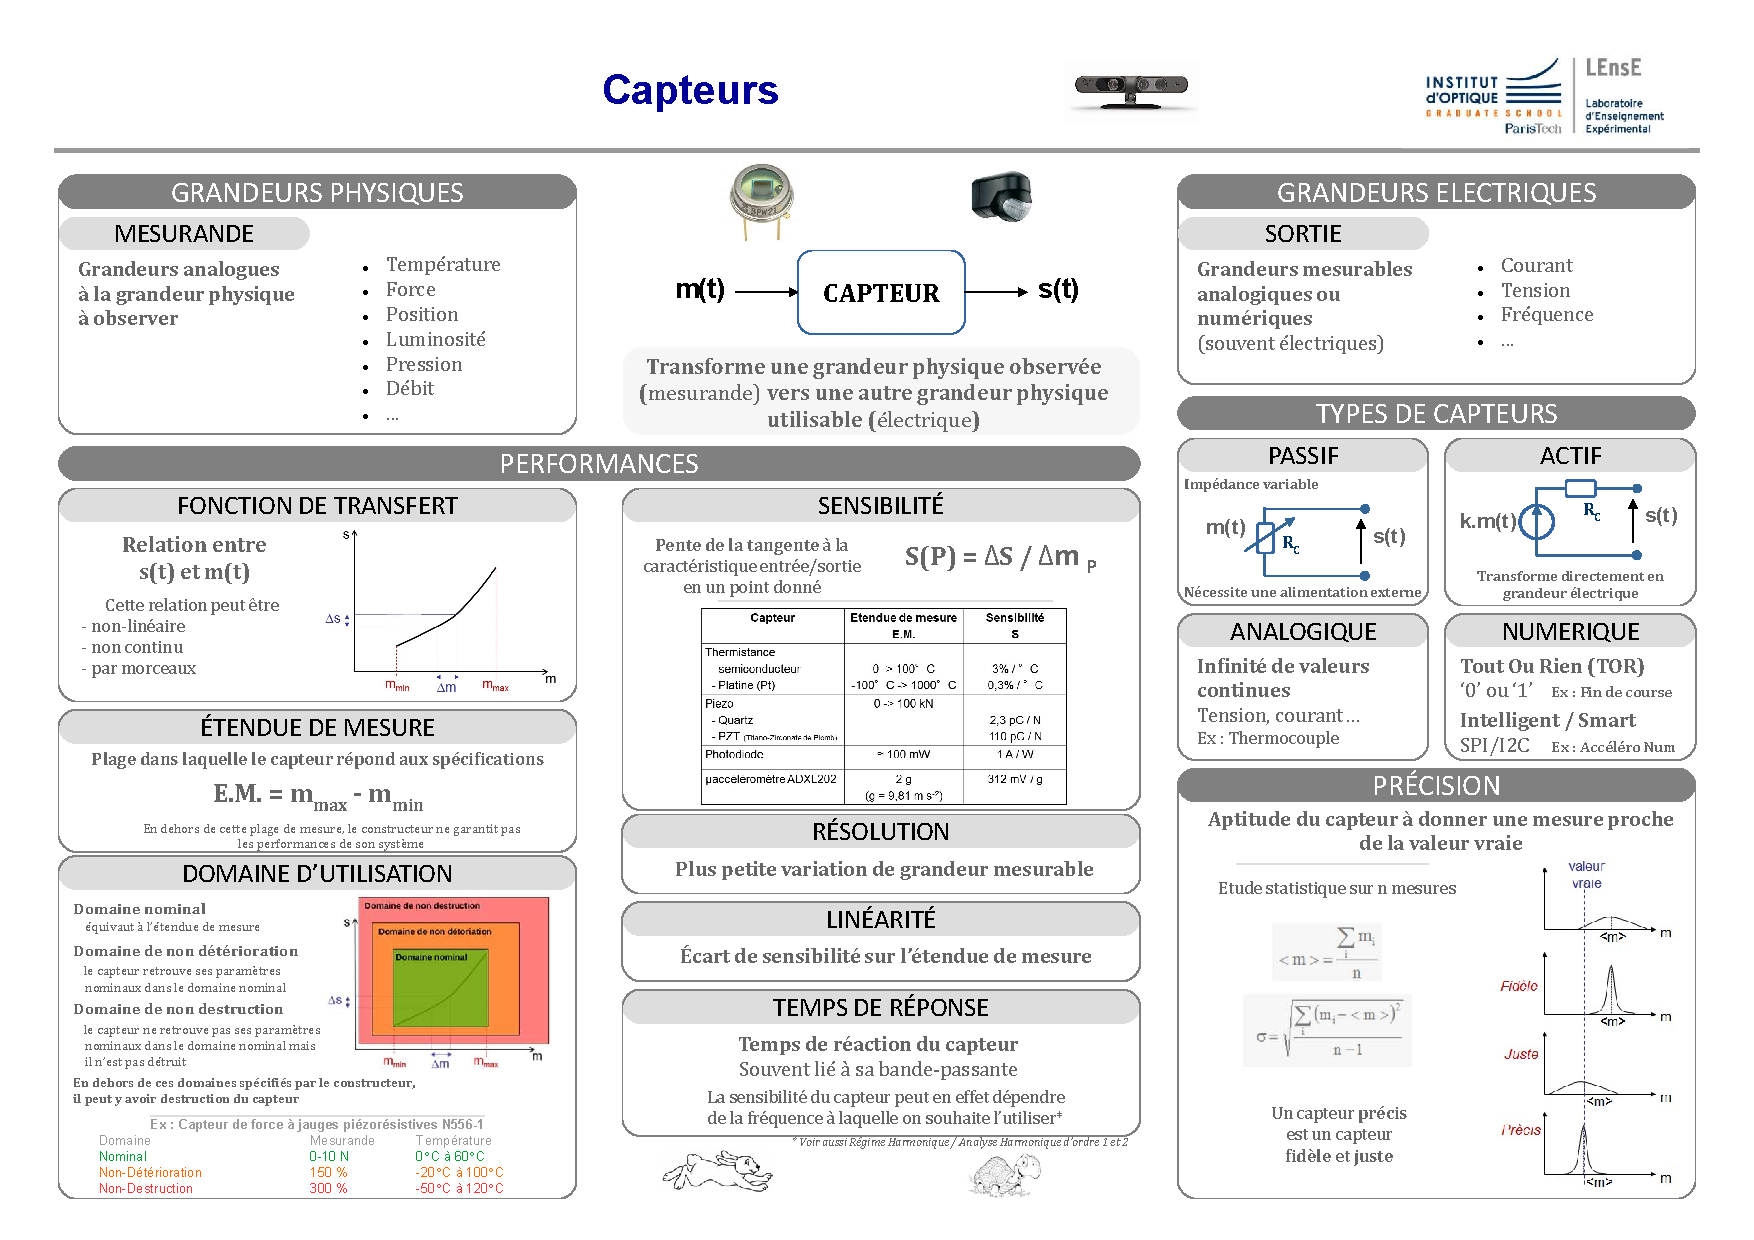
\includepdf[pages=-, landscape=true, pagecommand={\section{\texorpdfstring{\hspace{-1em}}{Fiche Bases}}}\label{fiche:Capteurs}]{../../../Fiches/Fiche_Capteurs.pdf}

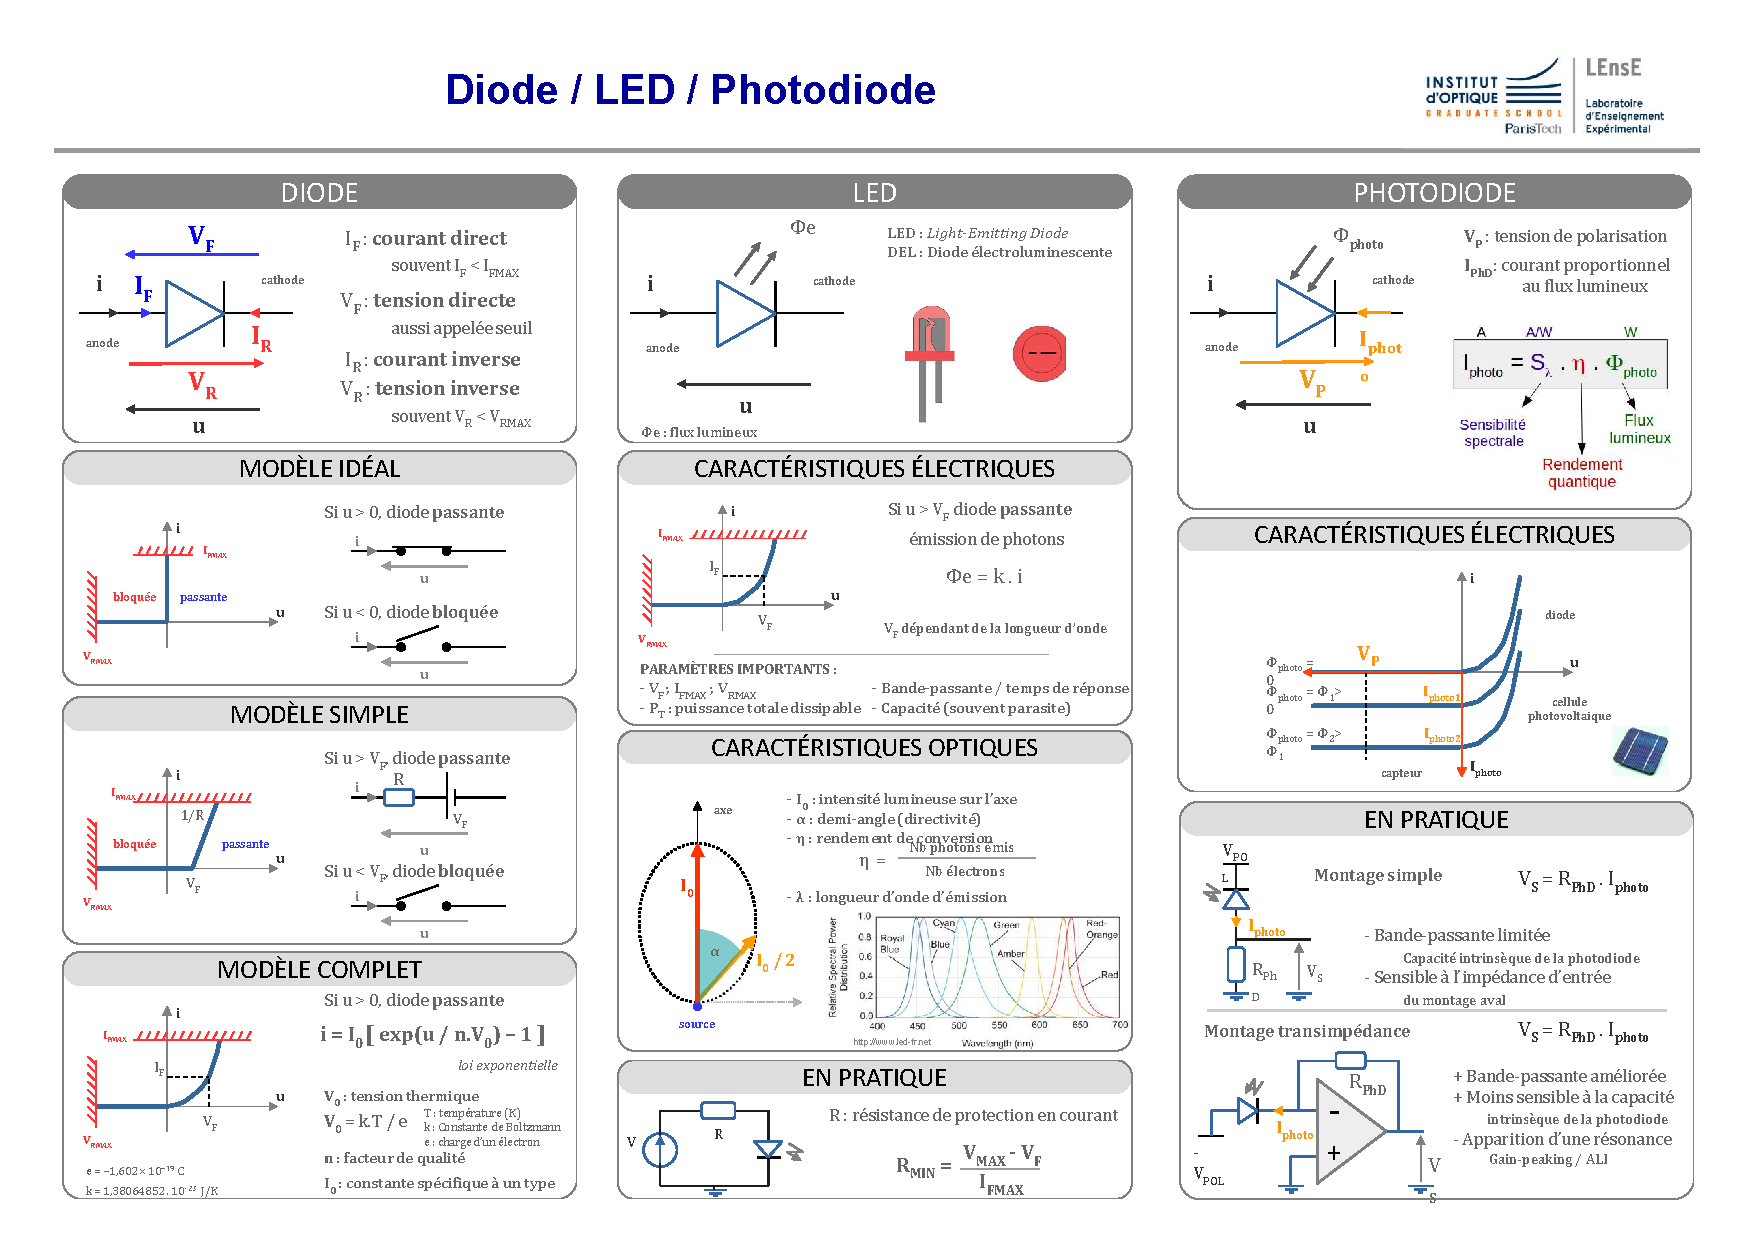
\includepdf[pages=-, landscape=true, pagecommand={\section{\texorpdfstring{\hspace{-1em}}{Fiche LED}}}\label{fiche:LED}]{../../../Fiches/Fiche_Diode_LED_Photodiode.pdf}

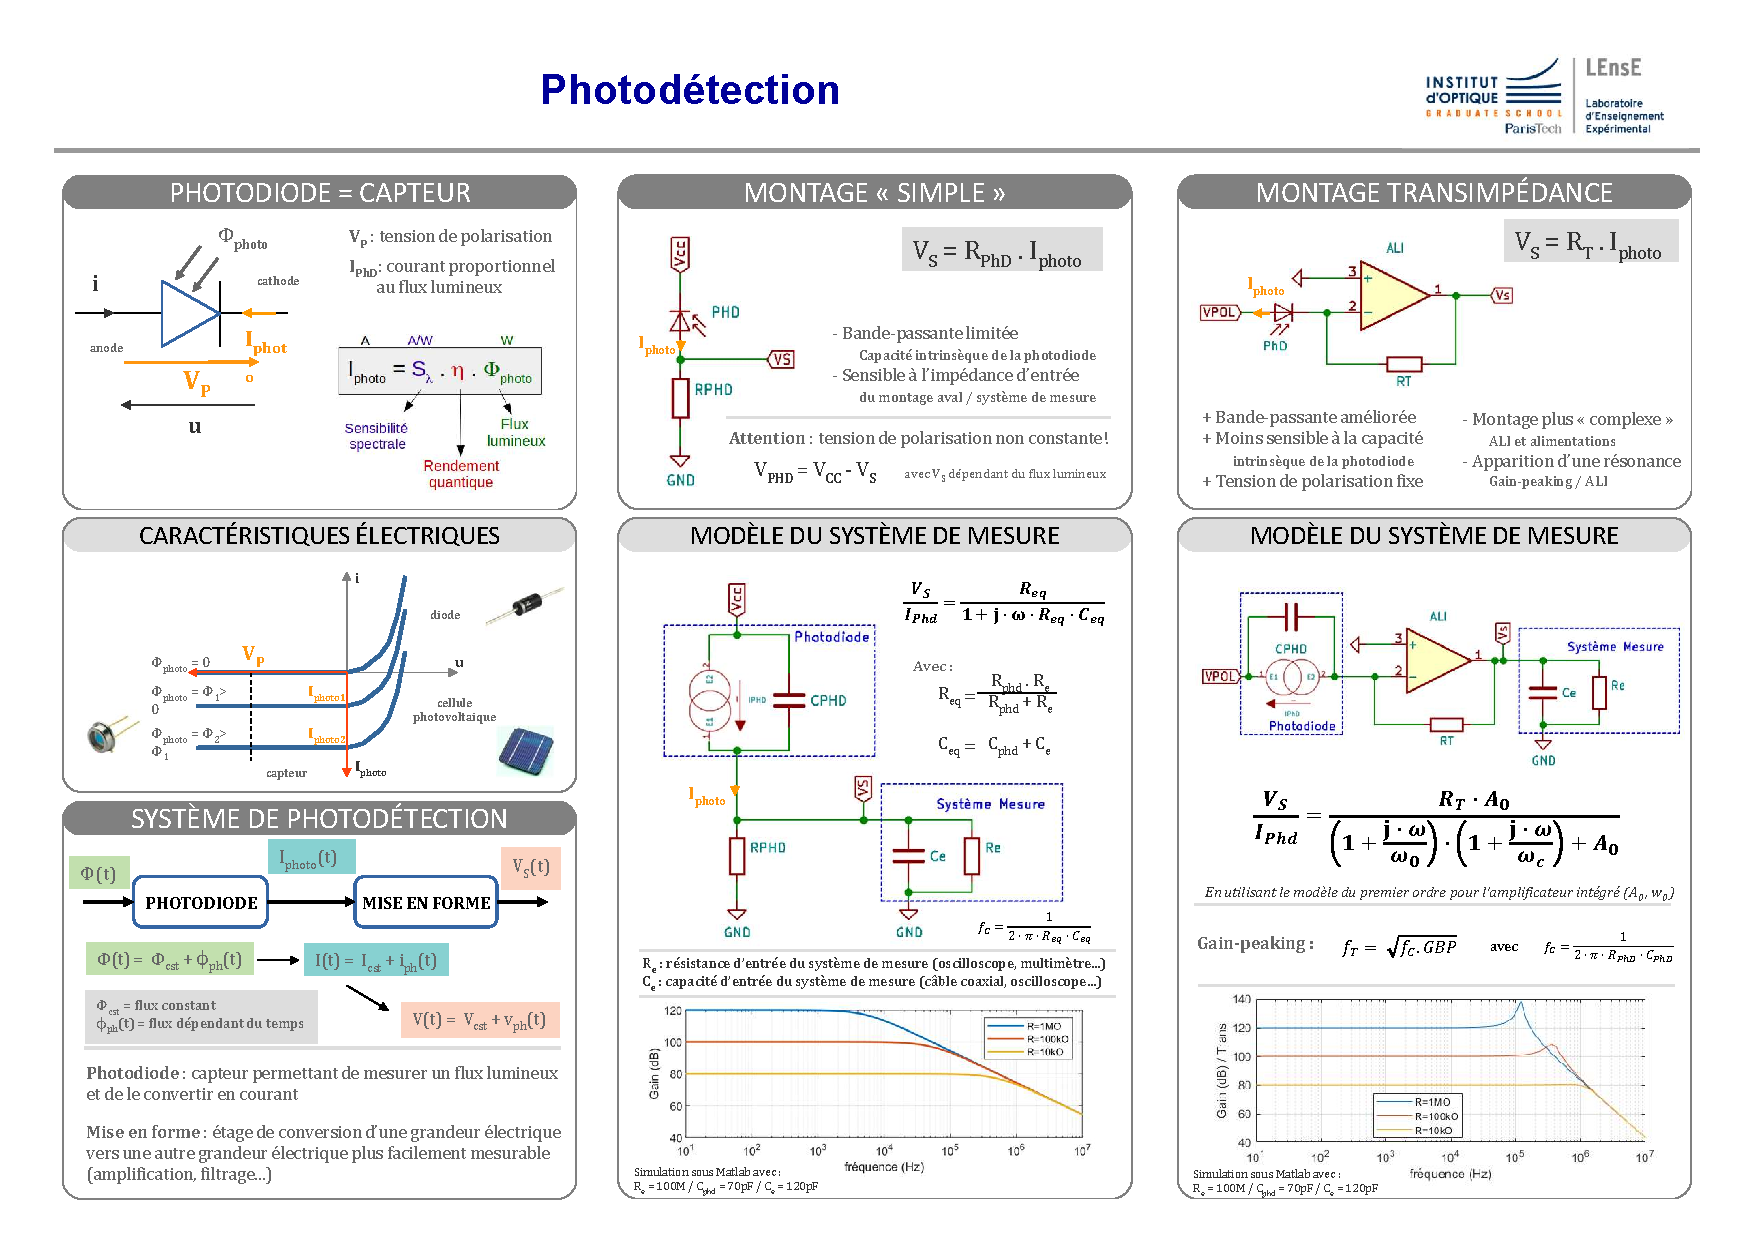
\includepdf[pages=-, landscape=true, pagecommand={\section{\texorpdfstring{\hspace{-1em}}{Fiche Photodetection}}}\label{fiche:Photodetection}]{../../../Fiches/Fiche_Photodetection.pdf}

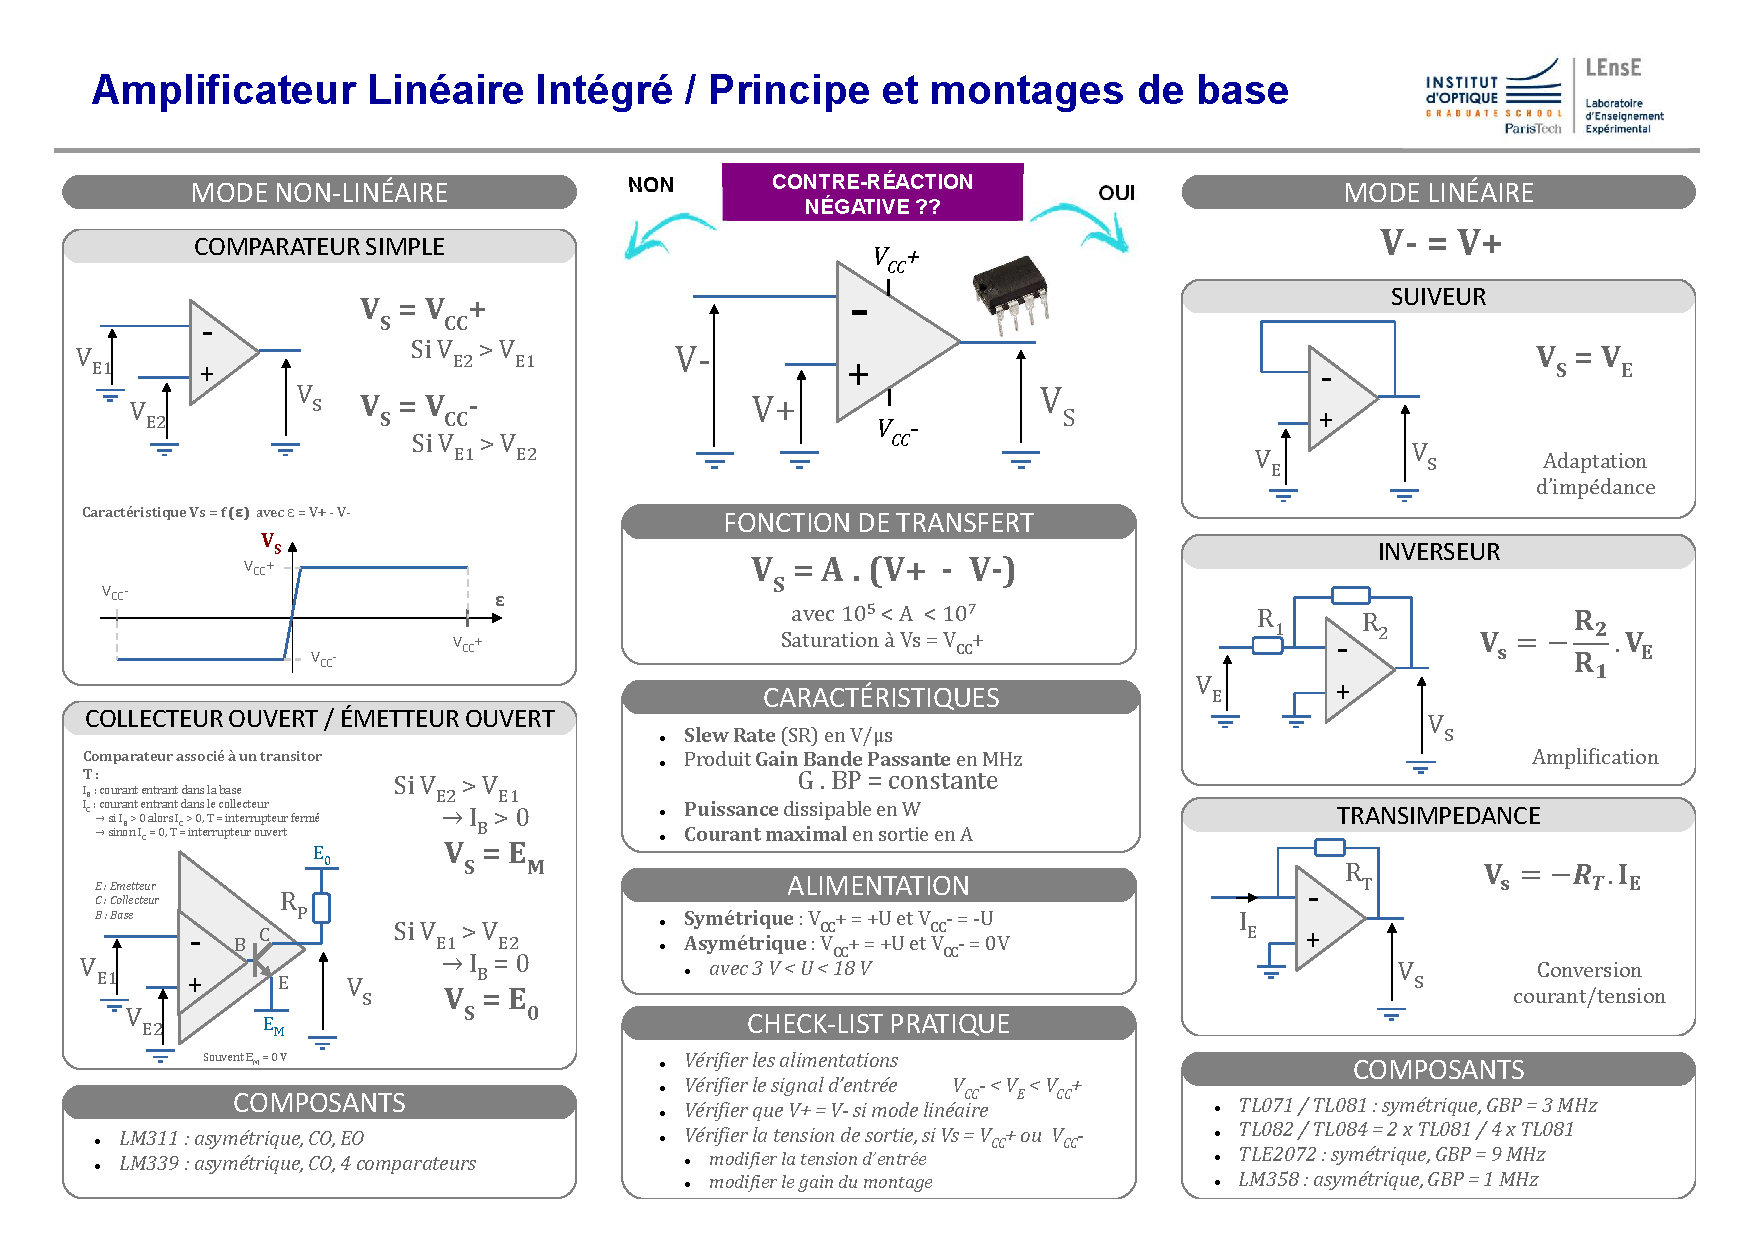
\includepdf[pages=-, landscape=true, pagecommand={\section{\texorpdfstring{\hspace{-1em}}{Fiche ALI}}}\label{fiche:ALI}]{../../../Fiches/Fiche_ALI.pdf}

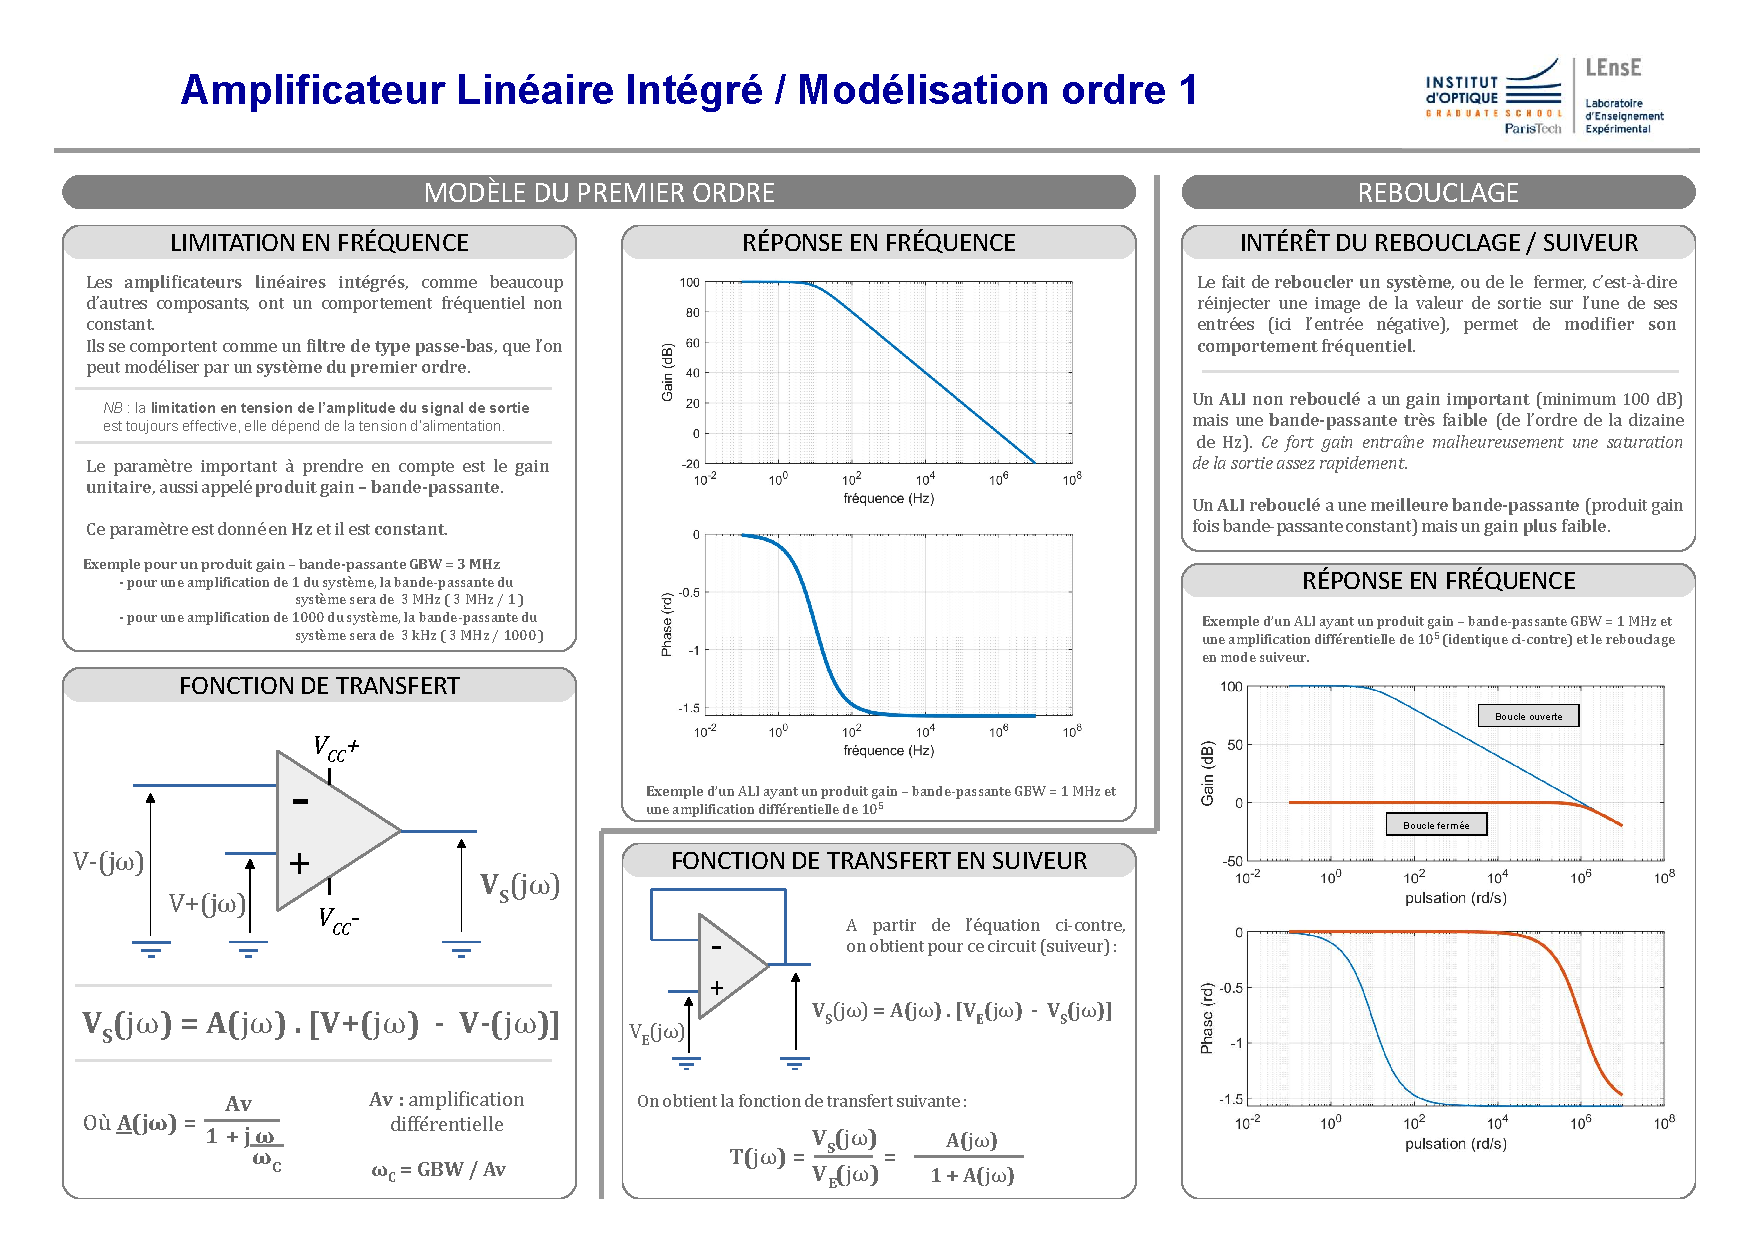
\includepdf[pages=-, landscape=true, pagecommand={\section{\texorpdfstring{\hspace{-1em}}{Fiche ALI Modele}}}\label{fiche:ALIModele}]{../../../Fiches/Fiche_ALI_Modele.pdf}

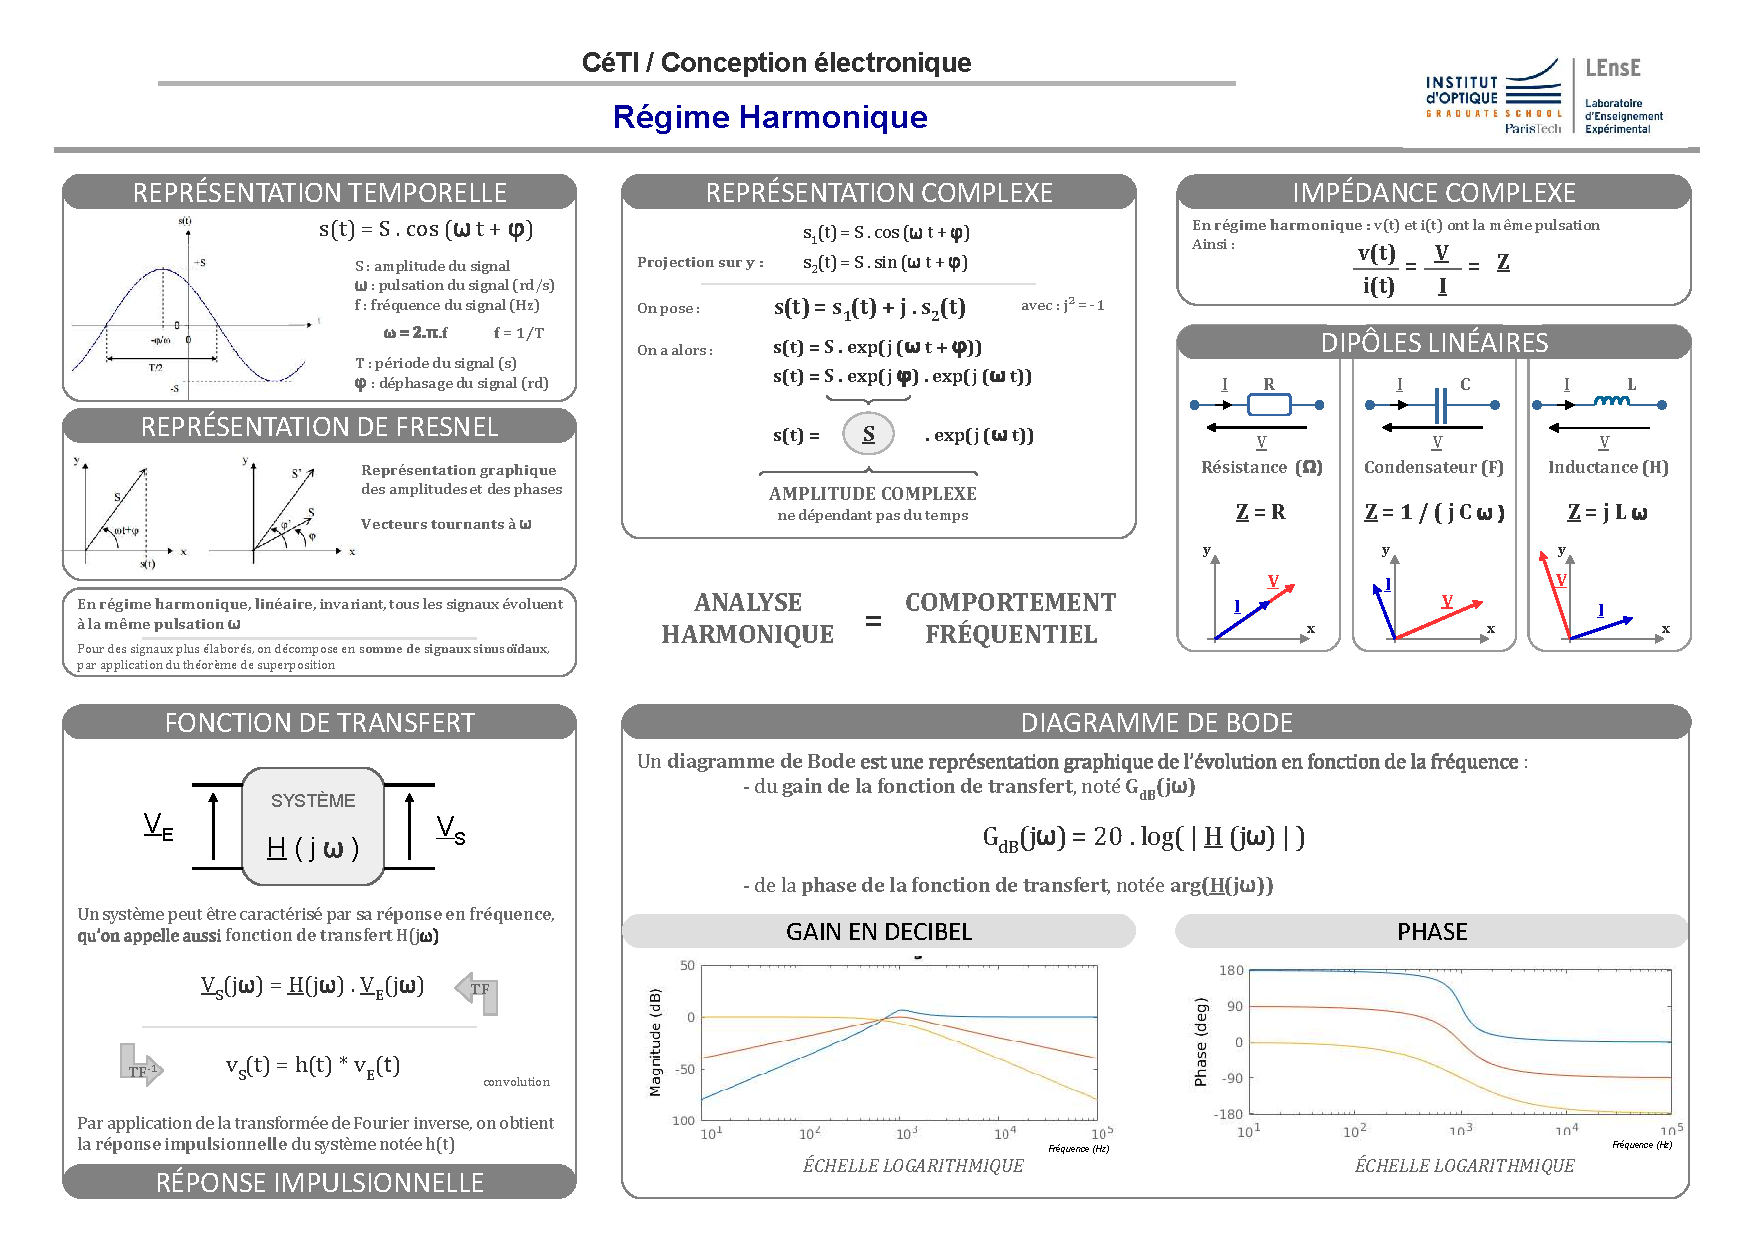
\includepdf[pages=-, landscape=true, pagecommand={\section{\texorpdfstring{\hspace{-1em}}{Fiche Regime Harmonique}}}\label{fiche:RegimeHarmonique}]{../../../Fiches/Fiche_Regime_Harmonique.pdf}


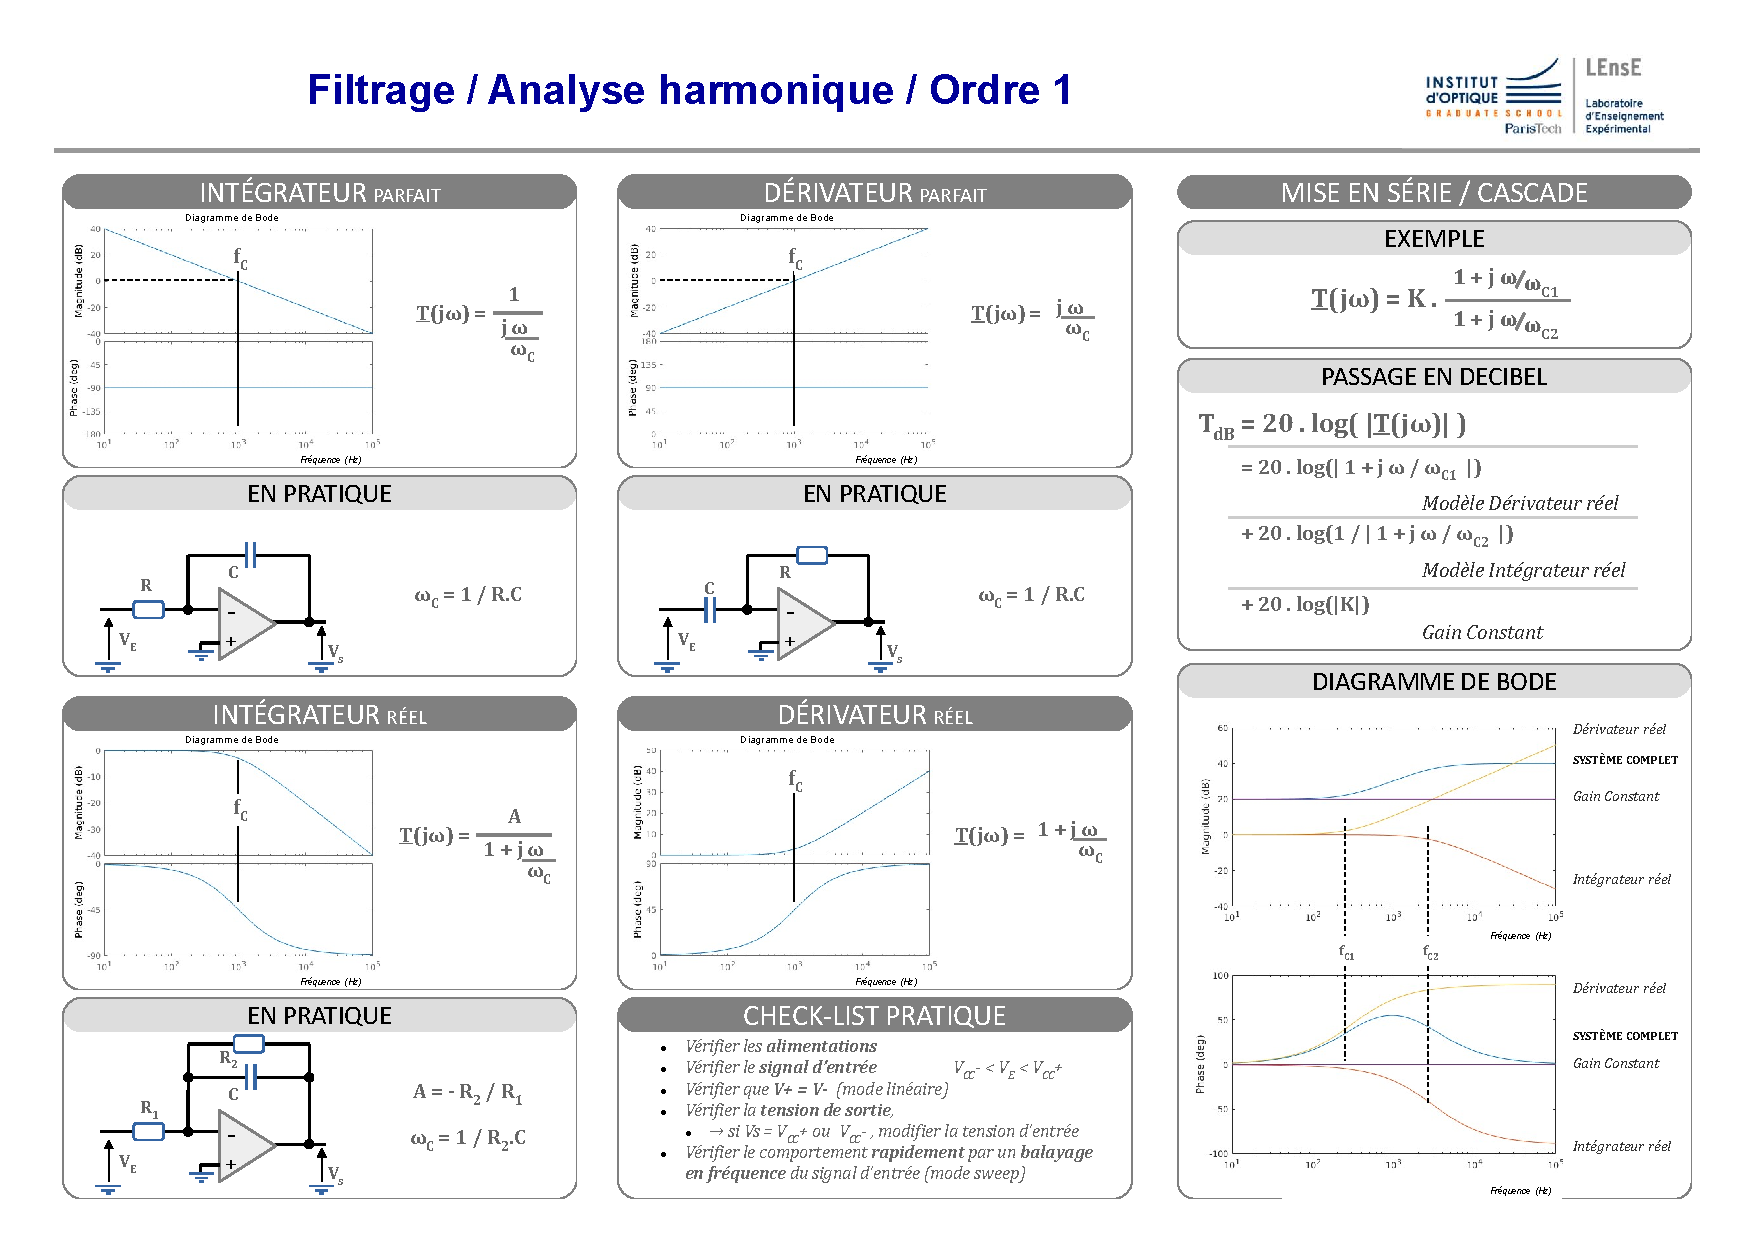
\includepdf[pages=-, landscape=true, pagecommand={\section{\texorpdfstring{\hspace{-1em}}{Fiche Analyse Harmonique Ordre 1}}}\label{fiche:AnHaOrdre1}]{../../../Fiches/Fiche_Analyse_Ordre1.pdf}

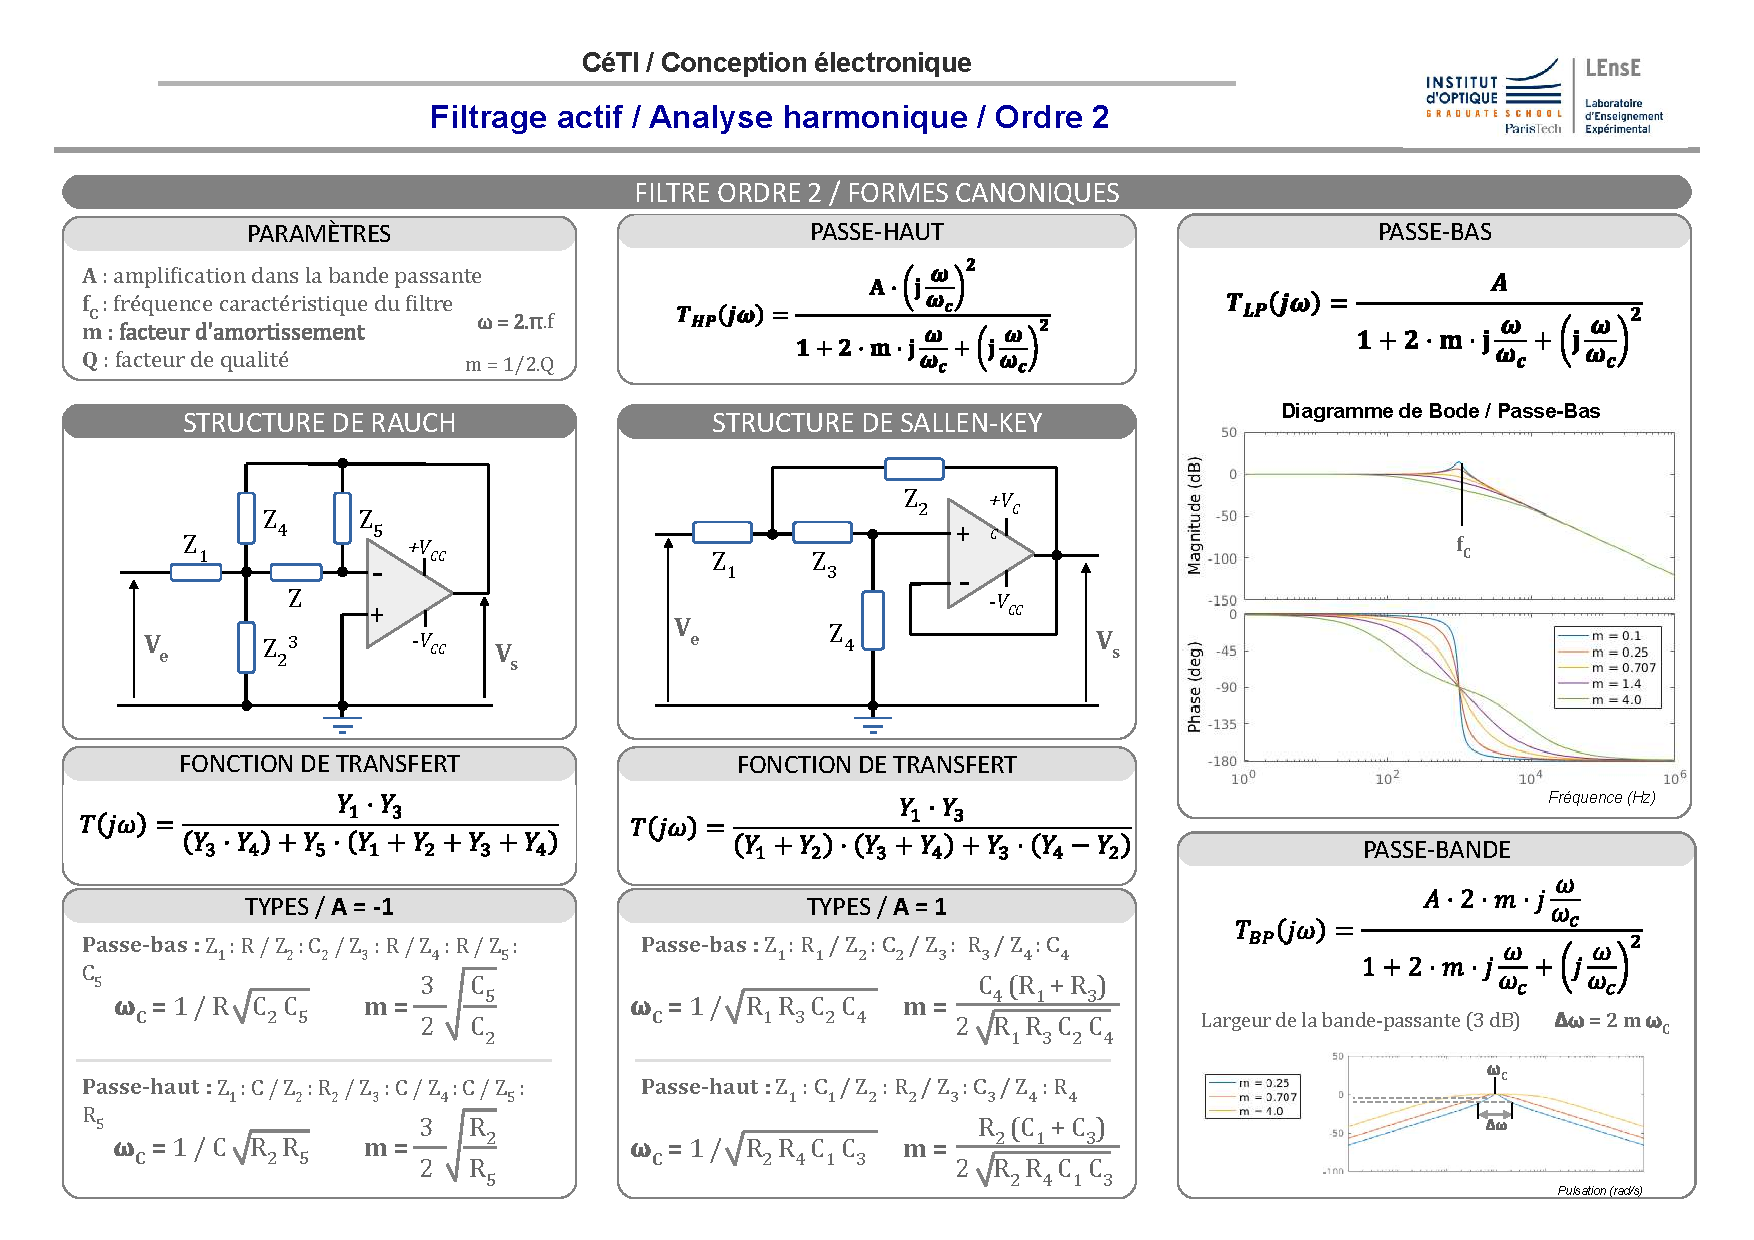
\includepdf[pages=-, landscape=true, pagecommand={\section{\texorpdfstring{\hspace{-1em}}{Fiche Analyse Harmonique Ordre 2}}}\label{fiche:AnHaOrdre2}]{../../../Fiches/Fiche_Analyse_Ordre2.pdf}


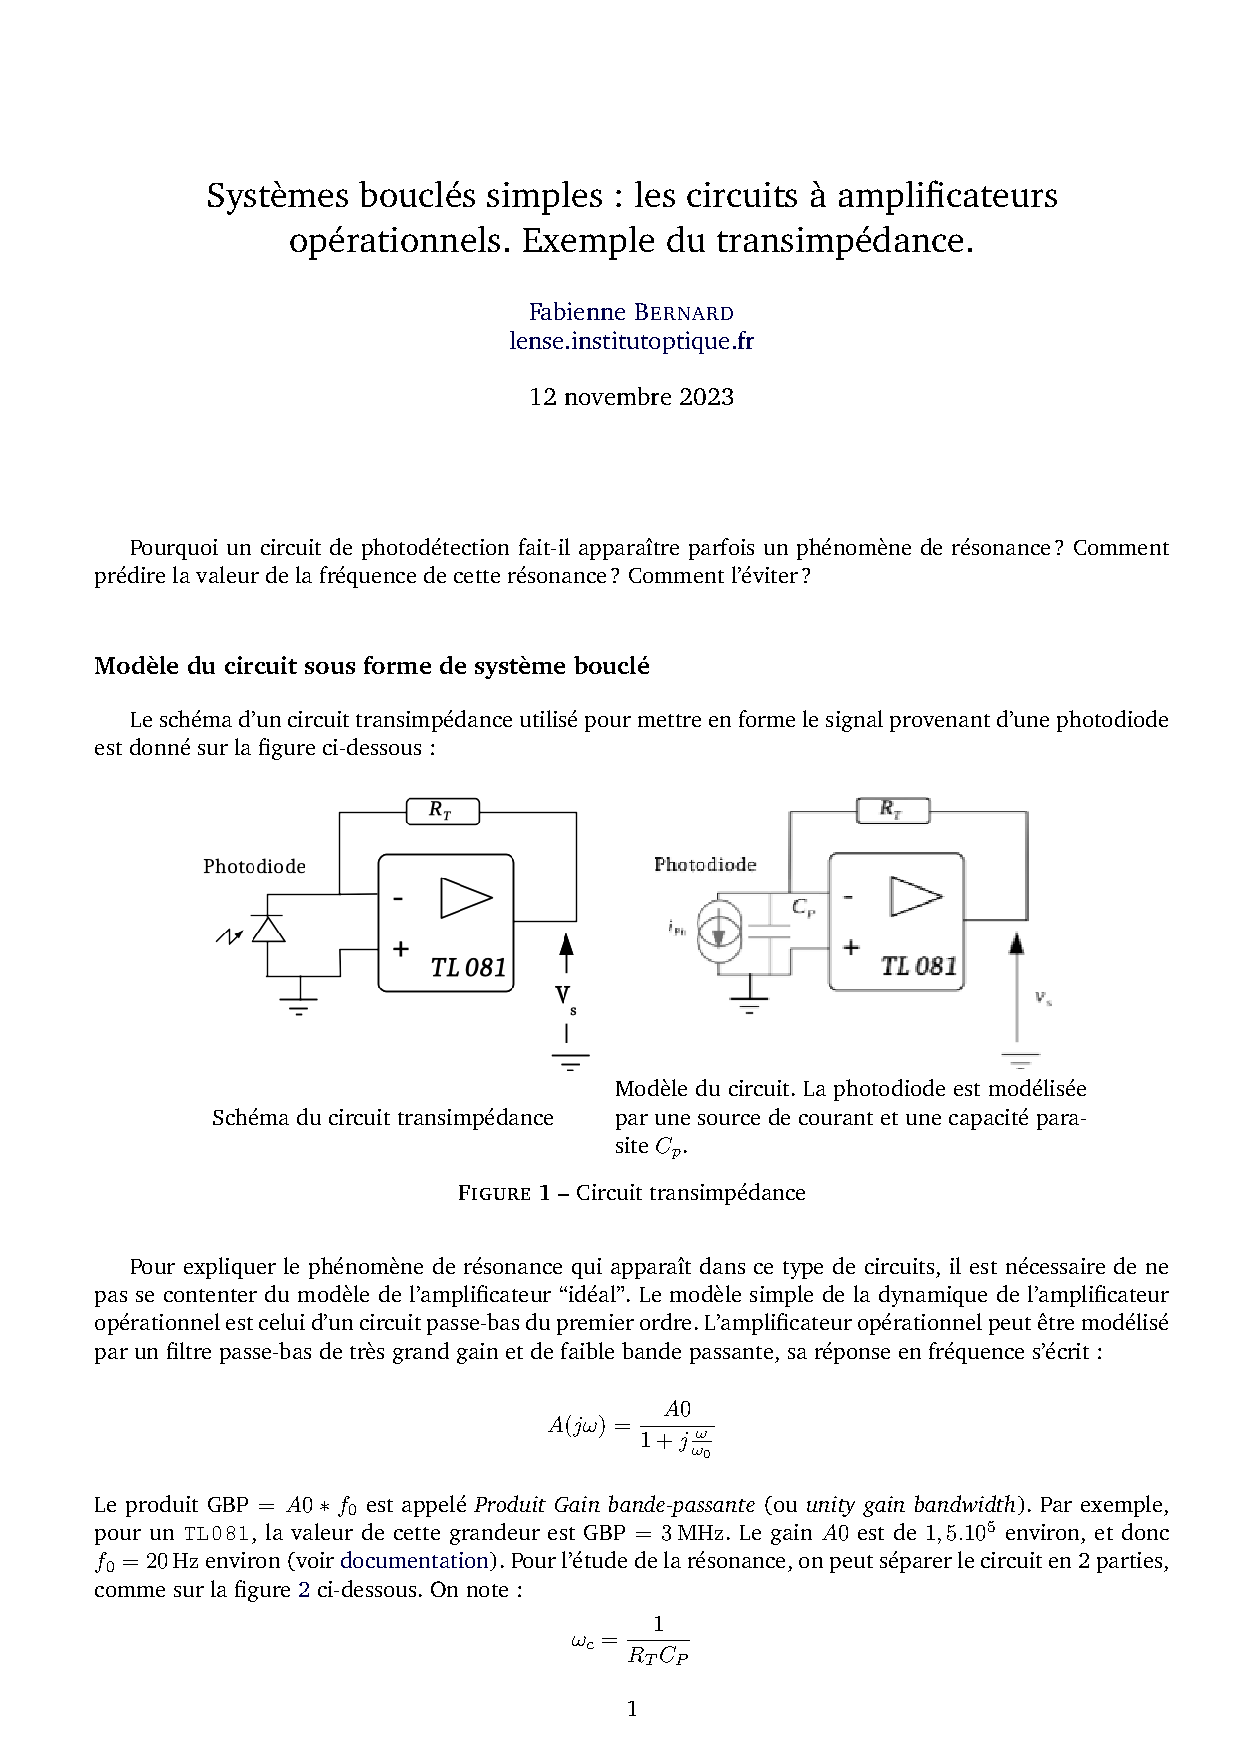
\includepdf[pages=-, pagecommand={\section{\texorpdfstring{\hspace{-1em}}{Modèle transimpédance}}}\label{fiche:ModeleTransimpedance}]{ressources/AnnexeTransImp.pdf}

\end{document}


